%#BIBTEX pbibtex YodaMT
\documentclass[12pt]{jarticle}
\usepackage{amsmath,amssymb} 
\usepackage[dvipdfmx]{graphicx,color} 
\usepackage{Soturon_ptex}
\usepackage{bm}
\usepackage[hang,small,bf]{caption}
\usepackage[subrefformat=parens]{subcaption}
\captionsetup{compatibility=false}
%\usepackage{slashbox}
%\usepackage{comment}
\renewcommand{\figurename}{Fig}

\newcommand{\tenti}{{\rm T}}
\setcounter{secnumdepth}{4}
%======諸設定======%
\isfinal{1}
%==================%
\title{歩行と走行のシンプルモデルに基づく2脚ロボット}
\author{世田 竜士}
\supervisor{細田 耕 教授}
\deadline{平成31年 1月 28日}


%==================%

\begin{document}
\setlength{\abovecaptionskip}{0mm}
% ===================タイトル======================
\titlepage
% ===================概要========================
\begin{abstract}
 2脚ロボットによる歩行や走行の研究は,ロボティクスの分野において数多く行われている.
これらの手法の1つに,
\end{abstract}
% ===================目次========================
\tableofcontents
% ===================本文========================

\section{序論}
近年,ヒトのような二足歩行や二足走行をロボットで再現する研究が行われており,安定な歩行や走行を実現した例が多く存在する.
Narioka et al.は,矢状面,前額面,水平面にロボットの運動を分割し,制御パラメータの探索を行うことで,3次元歩行を実現した\cite{pneumatbt}. % pneumat-bt
Ogawa et al.は,ヒトの3次元的筋配置を模倣したロボットを開発し,実際のヒトの筋電図に基づいた歩行モーションの再現により,3次元歩行を実現した\cite{pneumatbs}. % pneumat-bs % ここまで歩行
Niiyama et al.は,ヒトの下半身の筋骨格構造を模倣したロボットを開発し,ヒトの筋電図に基づきロボットの運動を制御することで,走行を実現した\cite{athleterobot}. % athlete robot % ここから走行
Raibert et al.は,1脚跳躍ロボットの位置制御を2脚ロボットの制御に拡張することで,二足走行を実現した\cite{Raibert:2000:LRB:518526}. % legged robots that balance
これらの研究に共通しているのは,ロボットの姿勢安定性ではなく,運動の持続性を維持することに着目することで,単純な制御則で歩行あるいは走行を実現している点である.

単純な制御則のみを用いてヒトのような運動を実現する手法として,簡略化されたモデルに基づく手法がある.
この手法を用いることで,ヒトの3次元運動を平面に分割し,制御性を向上させることができるという利点がある.
実際に,従来のロボットの研究では,ヒト特有の運動を説明可能なさまざまなモデルが提案されてきた.
その例が,歩行を表現する倒立振子モデル\cite{McGeer:1990:PDW:83528.83533,mobl,doi:10.1152/ajpregu.1977.233.5.R243}や,走行を表現するバネマスモデル\cite{BLICKHAN19891217,doi:10.1098/rspb.2006.3637}である.
これらのモデルを運動の制御に適用することで,ヒトの歩行及び走行の理解や,ロボットによる運動の実現に用いられてきた\cite{doi:10.1163/156855303321165097,893174,Seyfarth2547}.

一方,これまで提案されてきたモデルは,歩行と走行を異なるパラダイムとして扱ってきたため,同一のモデルで歩行と走行両方の運動を実現することは難しい.
そこで,Geyer et al.は,この問題を解決するために,走行の表現に用いられるバネマスモデルを拡張したモデルを考案し,歩行を説明しようとした\cite{doi:10.1098/rspb.2006.3637}.
提案されたモデルは,バネマスモデルに2本目の脚をつけることで,歩行と走行の両方を達成することであることを示した.
しかし,この拡張バネマスモデルでは,固有周波数が運動に大きく影響してしまう.
すなわち、ばね定数の調節によって速度を変化させることは可能であるが,それと同時に,歩行速度や足の接地点,脚の切り替え速度も変化してしまう.
このため,拡張バネマスモデルは,歩行モデルの制御や,従来の歩行モデルを説明するためには用いることはできない.

ヒトの歩行と走行の2つの達成が困難な理由として、従来の歩行モデルを説明するためには,走行動作には含まれない,両脚支持期における支持脚と遊脚の切り替えを考慮する必要があることが挙げられる.
一方で,それぞれの歩容における重心軌跡に着目すると,受動的動作によって生じる下凸の放物線運動と,自発的動作によって行われる上凸の放物線運動を周期的に繰り返す,共通の特徴を有している.
この共通項において,走行における制御則を歩行に拡張することで,2つの運動における脚の動作を同時に説明できる可能性がある.
そこで,本研究では,歩行運動と走行運動における共通項に着目し,進行方向への速度変化によって歩容を変化させることが可能な制御モデルを提案することと,その制御モデルに基づくロボットを試作することを目的とする.

本論文は,以下のような構成となっている.
2章では,目標速度の変化によって,歩行と走行の遷移が実現可能なモデルを提案し,シミュレーションにおける歩容の変化を示す.
3章では,2章で提案したモデルを再現するために試作したロボットの説明を行い,4章でロボットを用いた実験の内容について述べる.
最後に5章で,本研究における結論を述べる.
\clearpage

\section{歩行・走行モデル}
本章では,本研究で提案する,歩行と走行の両方を達成することが可能なモデルについて説明する.
これまで提案されてきたモデルでは,歩行運動は倒立振子モデルを用いて説明され,走行運動はバネマスモデルを用いて説明されてきた.
今回提案するモデルは,これら2つのモデルにおける共通項に着目している.
このため,まずそれぞれのモデルについての説明を行う.

\subsection{倒立振子モデル}
まず,歩行モデルである倒立振子モデル(Fig.\ref{ip})について説明する.
倒立振子とは,質量体に,質量を持たず変形しない脚がついたモデルである.
特に,質量体に同じ角度の間隔で脚をつけたモデルをリムレスホイールモデルといい,ヒトの歩行の重心軌道を表すことができる\cite{doi:10.1080/02681119708806242}.
Fig.\ref{rw}にリムレスホイールモデルを表した図を示す.
このモデルの運動は,次式のラグランジュ運動方程式によって説明することができる.
\begin{gather}
  L = \frac{1}{2}J\dot{\theta}^2 - mgl\cos{\theta} \\
 T = \frac{d}{dt}\frac{\partial L}{\partial \dot{\theta}} - \frac{\partial L}{\partial \theta} \\
 J\ddot{\theta} - mgl\sin{\theta} - T = 0 \\
 \frac{d}{dt} \left[
    \begin{array}{cc}
      \theta \\
      \dot{\theta}
    \end{array}
  \right] = \left[
    \begin{array}{cc}
      0 & 1 \\
      \frac{mgl}{J} \sin{\theta} & 0
    \end{array}
  \right] + \left[
    \begin{array}{cc}
      0 \\
     \frac{1}{J}
    \end{array}
  \right]
\end{gather}

ここで,\(L\)はラグラジアン,\(J\)は慣性モーメント,\(g\)は重力加速度である.

このモデルでは,ヒトの歩行において,単脚支持期における重心軌道や,支持脚長がほとんど変化しない点を再現できている.
特に,重心軌道に関しては,単脚支持期には上凸の放物線軌道を,両脚支持期には下凸の放物線軌道の動きを表し,これを周期的に繰り返す.
ここで,両脚支持期は,適切な加速度を与えるための力である,慣性力や蹴り出しの力を与える必要があるため,自発的な運動であるといえる.
逆に,単脚支持期では,与えられた慣性にしたがって重心を移動させる,受動的な運動であると捉えることができる.

\begin{figure}[htbp]
 \centering
 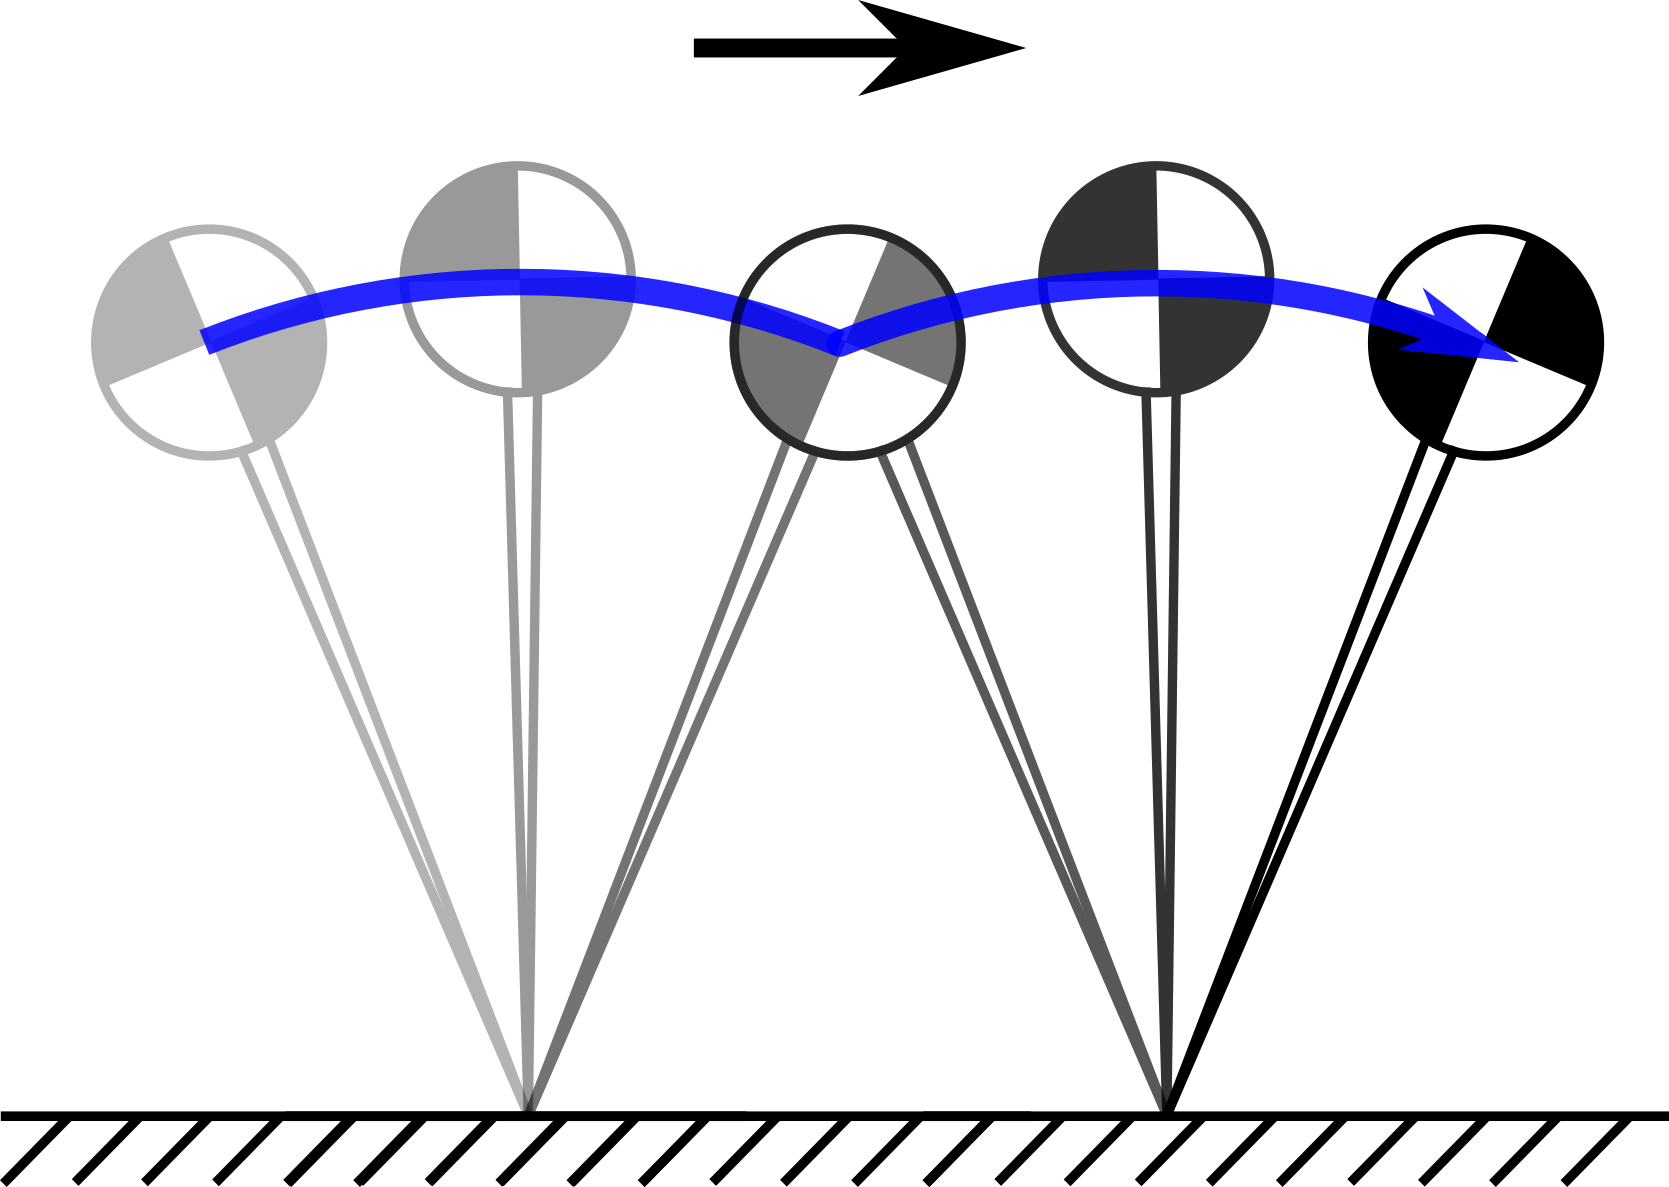
\includegraphics[clip,width=10.0cm]{./fig/inverted_pendulum_walking.png}
    \caption{倒立振子モデル.\label{ip}}
\end{figure}


\begin{figure}[htbp]
 \centering
 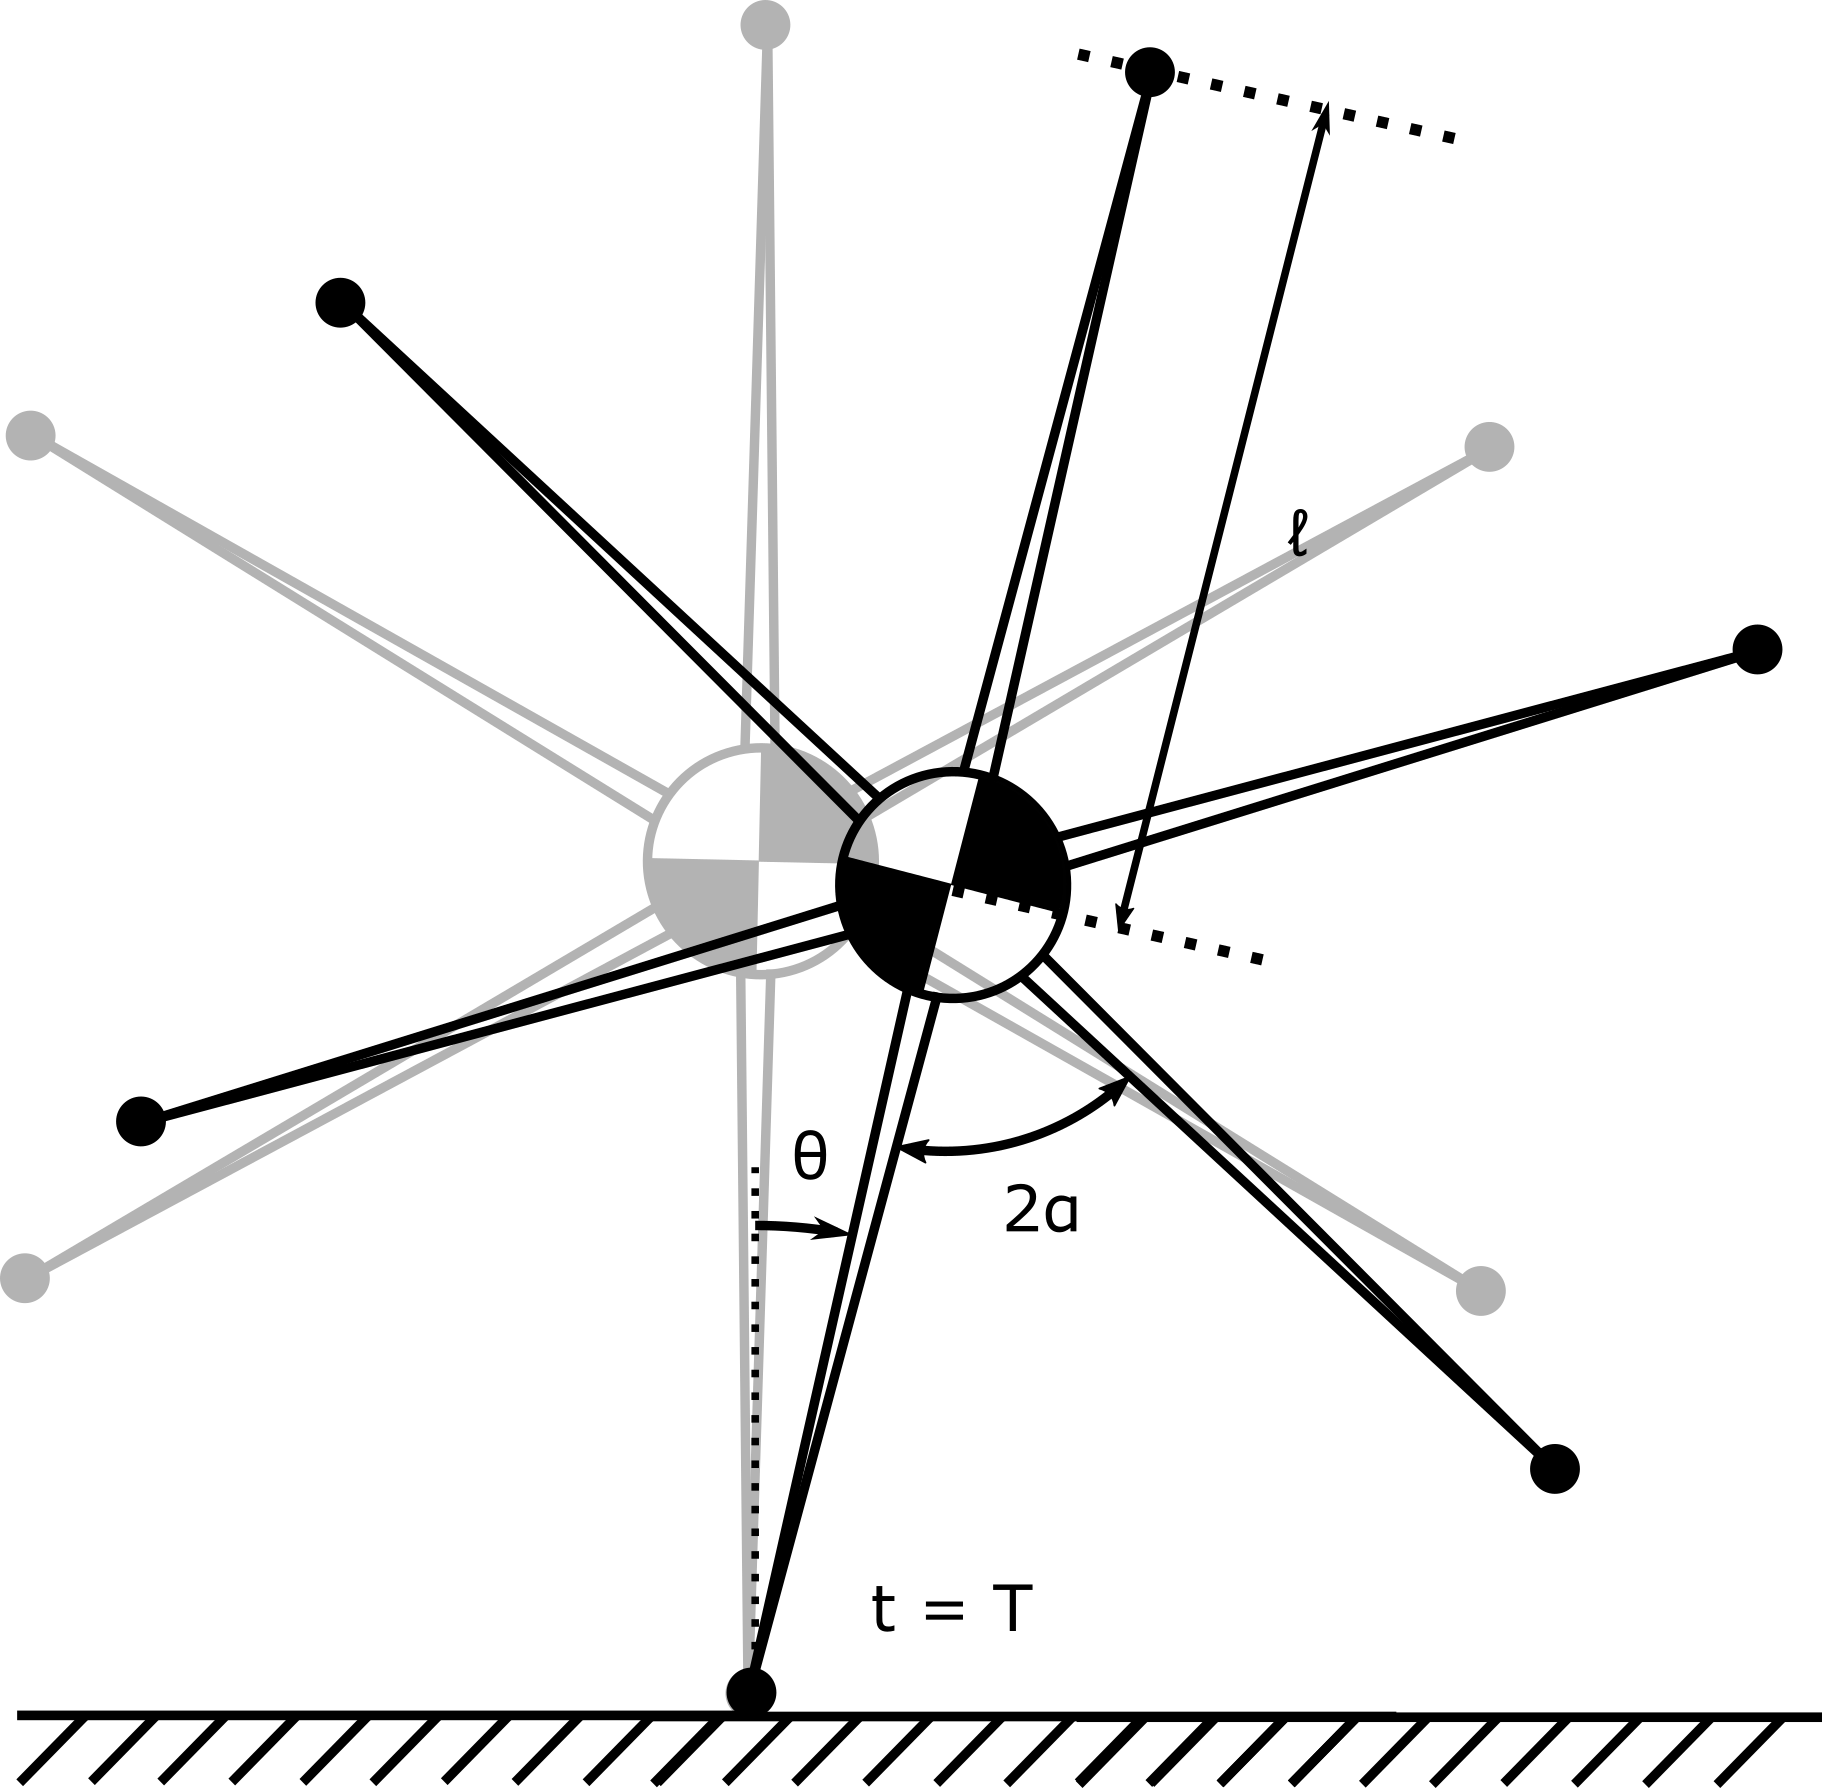
\includegraphics[clip,width=10.0cm]{./fig/rw.png}
    \caption{リムレスホイールモデル.\label{rw}}
\end{figure}



\subsection{バネマスモデル}
次に,走行モデルであるバネマスモデル(Fig.\ref{springmass})について説明する.
このモデルは,質量体に,脚方向に伸縮可能な柔軟なばね脚がついたモデルである.
倒立振子モデルでは,地面に着地したとき脚は変形しない.
それに対し,バネマスモデルでは,着地の際に脚が縮むことで,衝撃を吸収する.
着地の衝撃でばねに蓄えられたエネルギは,離地の際に利用され,跳躍のためのエネルギに変換される.
従来のバネマスモデルの制御手法は,鉛直方向と水平方向の2つに分けて制御を行っている.
鉛直方向の制御は,モデルの跳躍運動に関する制御であり,跳躍運動が脚の伸縮によりもたらされるものであることに着目し,跳躍運動の振幅を安定化させている.
水平方向の制御は,水平方向の移動速度に関する制御であり,接地位置を調節することで,移動速度を一定に保つ.
これらの鉛直方向の制御と水平方向の制御の繰り返しによって,走行を実現することができる.
このときの蹴り出しのために要するばねの力は,鉛直方向の制御則に基づき,次式のエネルギ保存則のように,目標高さによって算出される目標エネルギ\(E_{target}\)と,力学的エネルギによって算出される\(E\)の差によって定義することができる.
\begin{gather}
 E_{target} = mgy_{target} + \frac{1}{2}m \dot{x}_{target}^2 \\
 E = mgy + \frac{1}{2}m \dot{x}^2 + \frac{1}{2}m \dot{y}^2 + \frac{1}{2}kd^2
\end{gather}

ここで,\(y_{target}\)は目標高さ,\(\dot{x}_{target}\)は目標水平速度,\(d\)はばね定数である.
また,バネマスモデルの接地点は,水平速度\(\dot{x}\)と立脚期の長さ\(T_{stance}\)によって,次式で決定される.
\begin{gather}
 x_{f0} = \frac{\dot{x} T_{stance}}{2}
\end{gather}
さらに,この式に誤差訂正のためのPID制御を取り入れた次式によって,一定の速度での歩行が可能となる.
\begin{gather}
 x_{f} = \frac{\dot{x} T_{stance}}{2} + k_{\dot{x}} (\dot{x} - \dot{x_d})
\end{gather}

このときの跳躍時の水平方向の制御は,ばねによる力が働く上凸軌道を描く受動的な運動であり,立脚時の鉛直方向の制御は,慣性によって動く下凸軌道を描く自発的な運動であると考えることができる.

\begin{figure}[htbp]
 \centering
 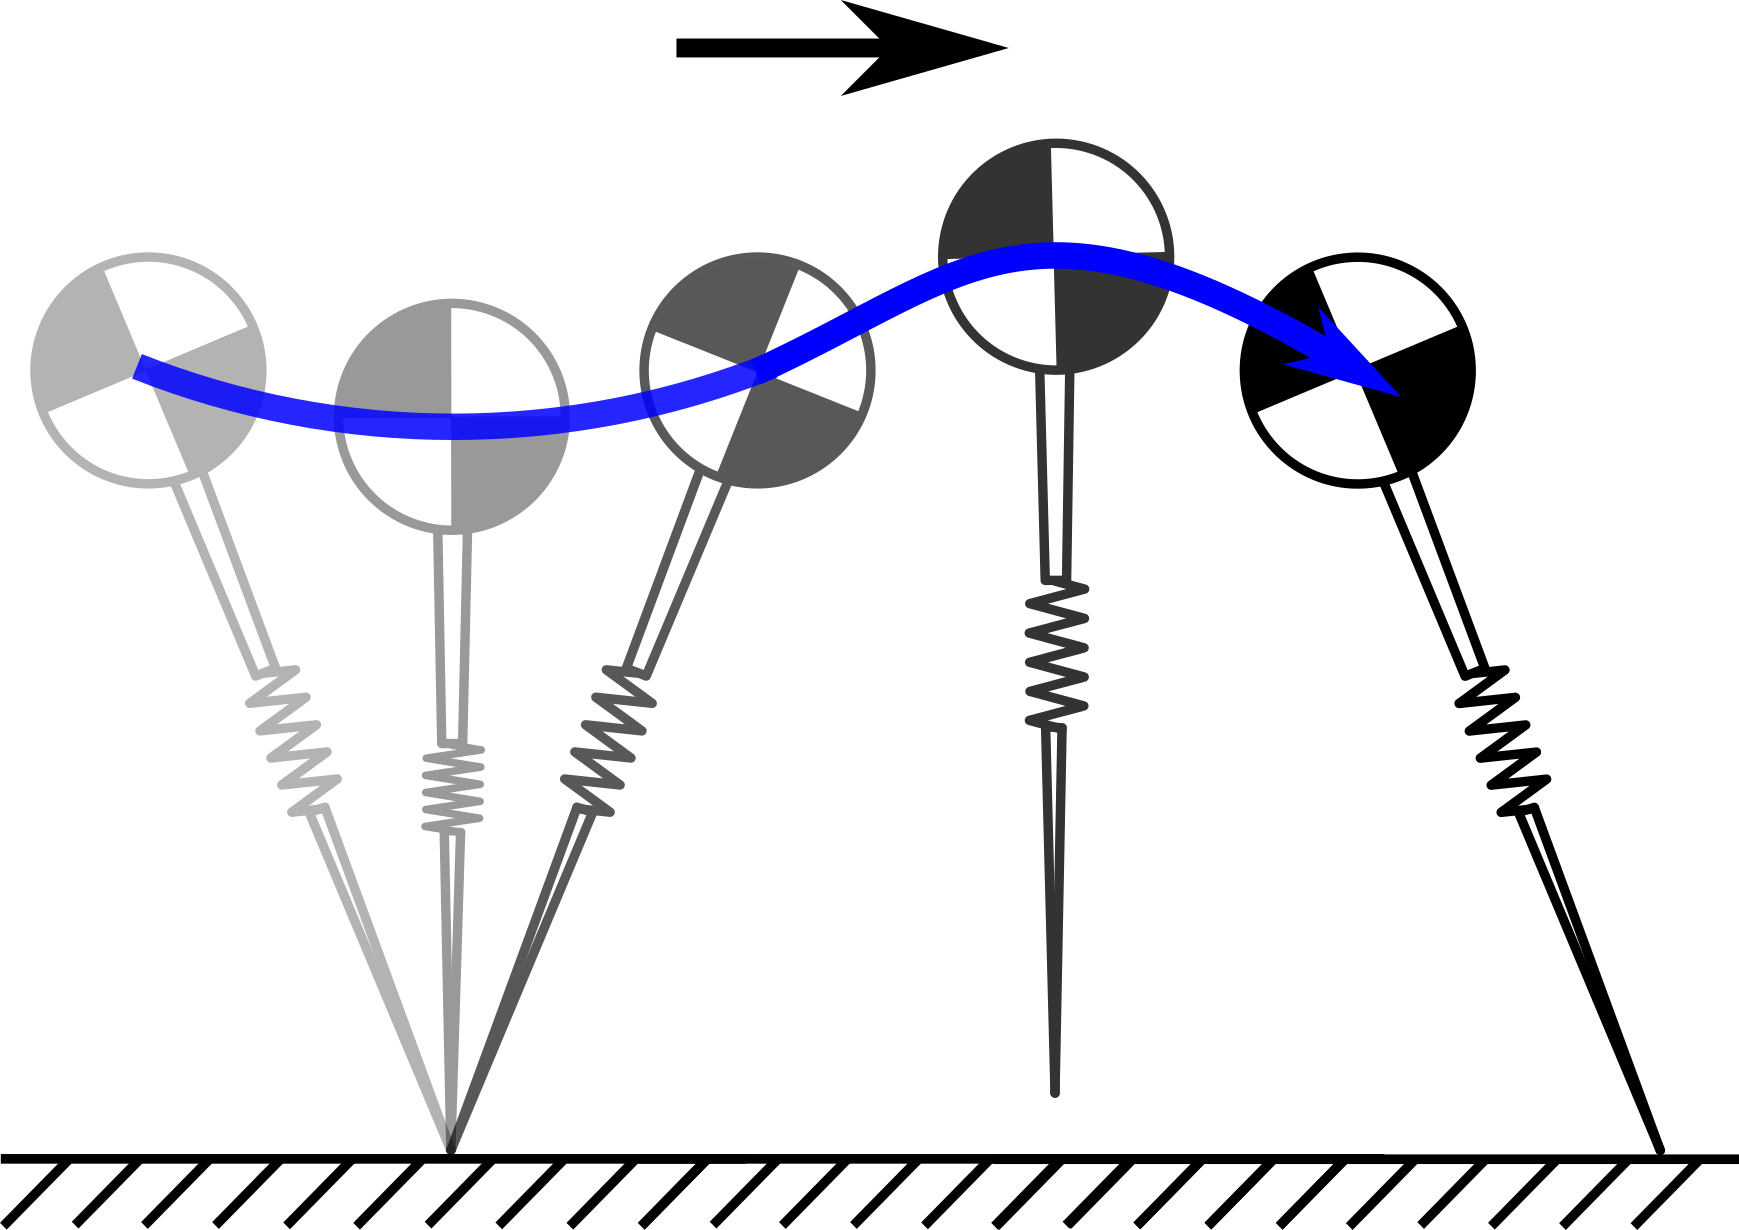
\includegraphics[clip,width=10.0cm]{./fig/slip_running.png}
    \caption{バネマスモデル.\label{springmass}}
\end{figure}



\subsection{提案する脚モデル}
本研究では,歩行時には倒立振子モデルのように振る舞う剛体脚を,走行時にはバネマスモデルのように伸縮可能な脚を同時に表現可能な脚モデルを考案した.
考案した脚モデルの構成をFig.\ref{model}に示す.
この脚構造は,ばね,ばねに作用するためのアクチュエータ,ダンパで構成されている.
また,脚はシリンダ部分とばね脚部分の2つに分かれており,ばね脚部分はシリンダ部分内に含まれている.
シリンダ脚部分は,上部にアクチュエータ,下部にダンパ物質が配置されている.
ばね脚部分には,ばねの上部と下部にストッパがついており,それぞれのストッパは,シリンダ上部にあるアクチュエータやシリンダ下部に接触する,又はどちらとも接触しない状態に変化することでそれぞれ,ばね脚,剛体脚,ダンパ脚のように脚構造の状態を変化させることが可能となっている(Fig.\ref{proposed_model}).
この脚構造の変化によって,歩行時は,シリンダ下部とばね脚の下部ストッパが接触し,後脚の蹴り出しと慣性によって前に進む倒立振子モデルのように振る舞う.
このとき,両脚支持期において,ばね脚部分はシリンダ内部に押し込まれて脚構造が収縮し,単脚支持への移行の際の推進力となる蹴り出し動作を生む.
このため,提案する脚モデルに見られる重心軌道は,倒立振子モデルに見られる両脚支持期の重心軌道とは形状がやや異なった下凸の放物線軌道を描く.
この放物線軌道は,走行動作の支持脚期における下凸の放物線軌道と一致することに注意したい.
また,走行時は,脚の収縮時にばね脚部分がシリンダ内に押し込まれて,シリンダ上部とばね脚の上部ストッパが接触することで,バネマスモデルのように振る舞う.

シリンダ下部にあるダンパ物質は,両脚支持期から単脚支持期への歩行周期の移行の際に重要な役割をもつ.
両脚支持期後期において,後脚は蹴り出しによって重心を押し上げるため,前脚は伸長し,シリンダ下部とばね脚下部ストッパは接触しようとする.
このとき,ダンパ物質が作用することで,接触と同時に発生する跳躍する力を減衰することができ,歩行運動の実現を可能としている.

また,ダンパ物質は,モデルのような直動式の脚構造だけでなく,ヒトのような回転式のリンク構造のにおける歩行の説明においても効果的に機能する.
直動式の脚構造において,脚が伸長するとき,脚方向へは一定の速さで伸長する.
一方,回転式のリンク機構では,関節が屈曲状態から伸展状態に移行するとき,脚方向への伸長率は,脚が伸展するほど低下する.
ダンパ物質を導入することで,直動式の脚構造においても,脚方向への伸長率の低下を再現することができる.

本研究では,このモデルを用いて,歩容を安定させる制御則を導入することで,歩行と走行の歩容の実現を目指す.

\begin{figure}[htbp]
 \begin{minipage}[b]{.5\linewidth}
 \centering
 
\includegraphics[width = 6.0cm, clip]{./fig/leg_cylinder.png}
 \subcaption{提案する脚モデルのシリンダ部分.\label{leg_cylinder}}
 \end{minipage}
 \begin{minipage}[b]{.5\linewidth}
 \centering
 
\includegraphics[width = 3.5cm,clip]{./fig/leg_spring.png}
 \subcaption{提案する脚モデルのばね脚部分.\label{leg_spring}}
 \end{minipage}
\caption{提案する脚モデルの構成.実際の運動中には,ばね脚部分はシリンダ部分に内蔵されている.\label{model}}
\end{figure}

\begin{figure}[htbp]
 \centering
 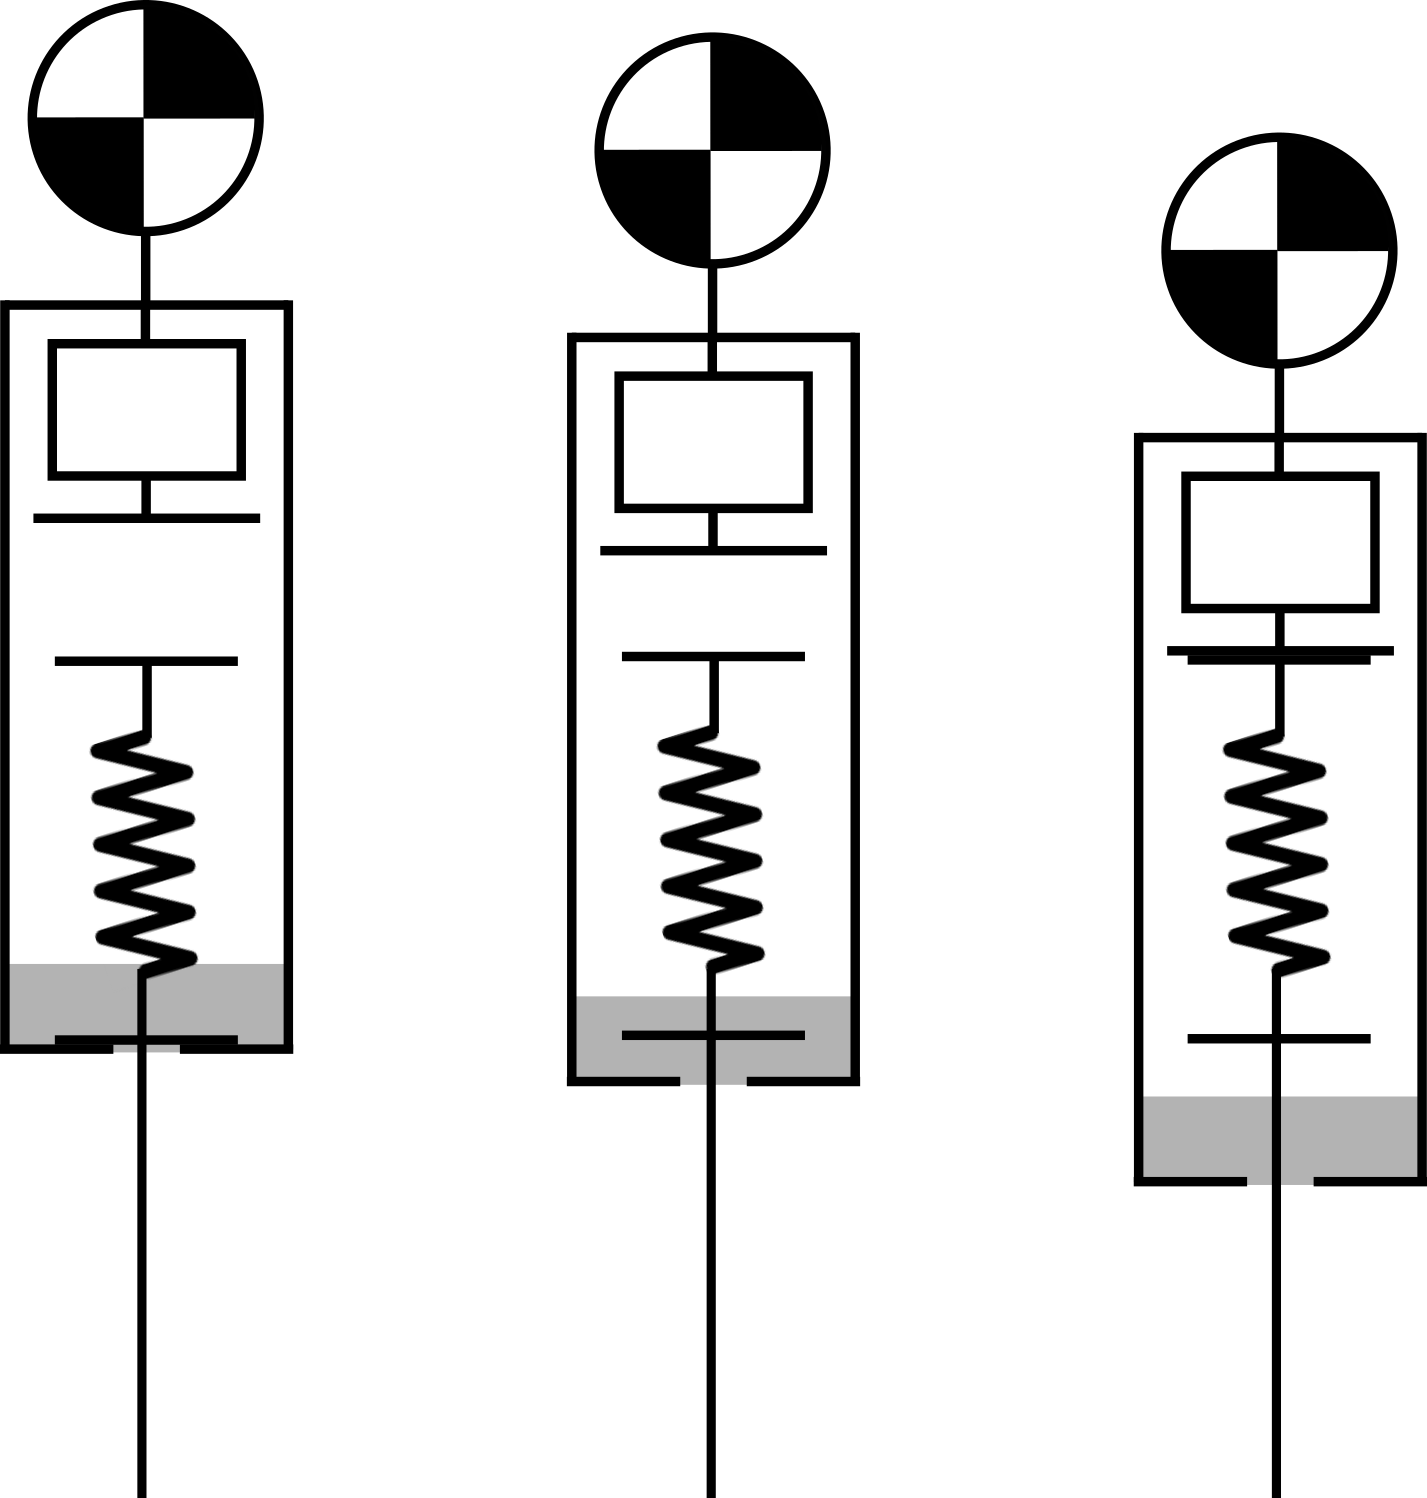
\includegraphics[clip,width=8.0cm]{./fig/leg_concept.png}
    \caption{提案する脚構造の脚状態.左から順番に,剛体脚,ダンパ脚,ばね脚の状態を表している.これらの脚の状態は,ばね脚部分の上部・下部につけられたストッパの位置によって決定される.\label{proposed_model}}
\end{figure}



\subsection{歩容制御アルゴリズム}
提案したモデルの制御則として,前述したバネマスモデルの安定化手法を拡張することを考える.
歩行モデルと走行モデルの2つで単脚支持期における挙動を比較すると,歩行モデルでは,脚の長さが変化しないために上凸軌道を描くのに対し,走行モデルでは,ばねが収縮するために下凸軌道を描く.
この動作の差異が原因で,歩行と走行を同時に表現することは難しい.
しかし,この下凸軌道の自発的運動と上凸軌道の受動的運動の繰り返しの現象は,前述したように,歩行の場合においても同様に見られる現象である(Fig.\ref{compare}).
すなわち,歩行運動と走行運動において,脚の伸縮動作中に水平方向の制御が働くという共通項がある.
この共通項に着目することで,走行における制御則を,歩行に拡張できる可能性があると考えた.

そこで,モデルの制御則として,仮想脚という概念を導入することで,歩行と走行の制御則を一般化することを考えた.
仮想脚の定義として,最大長を任意の長さに設定可能であり,歩行での両脚支持期における中間点にある,収縮可能な脚と仮定する.
仮想脚の脚長を,走行時の実際の脚長と仮定すると,モデルにおける仮想脚と実際の脚の動きは一致し,仮想脚は走行運動の動作を見せる.
歩行時は,仮想脚の自然長が,両脚支持期初期の質量体と各脚の中間点の長さと仮定すると,歩行中の仮想脚は,両脚支持期中は重心が低くなるために,走行動作
支持脚のような振る舞いをする.
また,単脚支持期には,仮想脚は収縮状態から自然長に伸びている状態であり,実際の脚より短い状態であるため,跳躍運動を行う.
これにより,歩行時における仮想脚は,走行動作のように支持脚期と跳躍期を繰り返すように振る舞う.
このように,仮想脚を想定することで,歩行と走行の2つの動作を,仮想脚の走行動作と同様に記述することができる.
走行動作の制御は,バネマスモデルにおいて使用される制御則を用いることで実現できる.
このため,本モデルで,仮想脚を想定し,モデルの仮想的な運動の制御を行う手法を用いる.

ここで,提案するモデルの実際に使用する制御において,実際の走行モデルと異なる,2つの制約条件を考慮する必要がある.
1つ目が,実際の脚と仮想脚の着地タイミングが異なる場合がある点である.
仮想脚を想定したモデルを考えたとき,仮想脚の定義した脚長によって,実際の脚が接地するよりも前に仮想脚が接地する場合が生じ得る.
その場合,実際の脚が接地するまで,仮想脚の位置が接地位置で固定されているものとして制御を行う.
2つ目が,仮想脚の状態の遷移に関する問題である.
単にこのモデルを使用するだけでは,歩行と走行を安定して行うことは可能だが,2つの動作を遷移することはできない.
実際の脚の歩容によって,仮想脚は異なる状態となる可能性を有している.
例えば,歩行動作中の場合,単脚支持期において,仮想脚は跳躍期になる.
一方で,走行動作中の場合,単脚支持期には,仮想脚は単脚支持期である.
このように,動作によって,実際の脚が単脚支持期中であるとき,仮想脚は単脚支持期にも跳躍期にもなりえる.
このため,歩容の遷移を可能とするために,2つの条件を制御に加える.
実際の脚による運動の状態が安定な状態であれば,仮想脚は,跳躍期と単脚支持期を周期的に繰り返す.
しかし,運動の状態が不安定な場合,歩容が歩行から走行に,または走行から歩行に変化する場合がある.
これを考慮するため,仮想脚は,跳躍期と単脚支持期の周期を2回繰り返すことによって,実際の脚の状態に合わせる必要がある.

これらの制約を考慮すると,以下の2つの条件を認める必要がある.

\begin{itemize}
 \item[\labelitemiv] 実際の脚が単脚支持期に移行したとき,仮想脚も別の状態に移行する.
 \item[\labelitemiv] 実際の脚が両脚支持期であるとき,仮想脚は単脚支持期に移行する.
\end{itemize}

これらの制約条件を制御則に組み込むことによって,歩容の遷移が可能になり,モデルでの歩行と走行の安定性を説明できるようになる.


\begin{figure}[htbp]
 \centering
 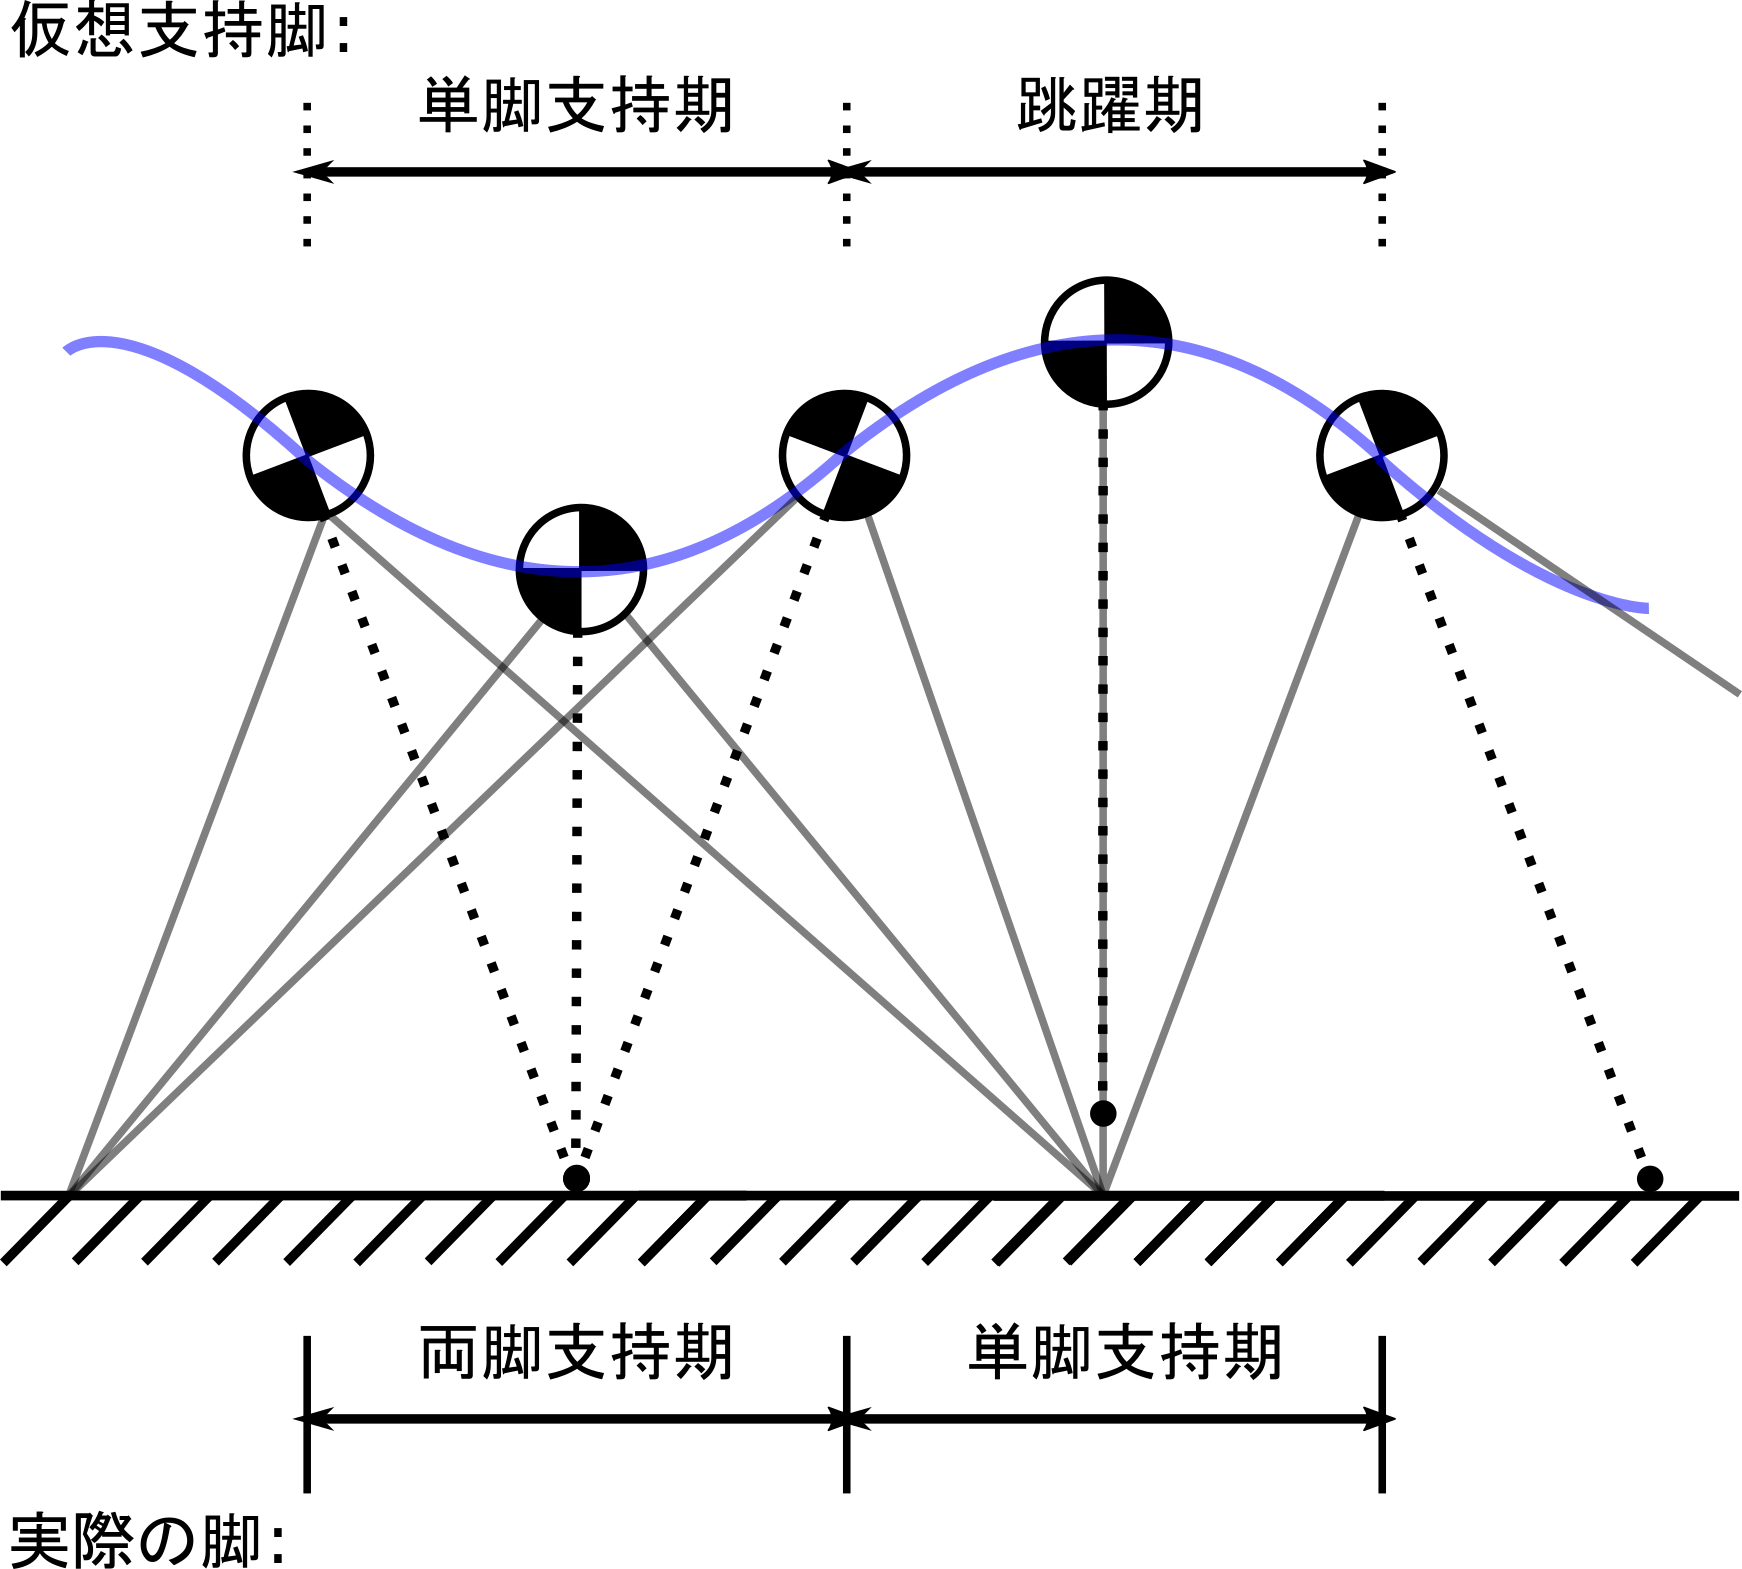
\includegraphics[width = 10.0cm, clip]{./fig/walking_with_vsl.png}
 \caption{歩行動作に仮想脚を導入した場合.青色の曲線は重心軌跡を,黒色の線は脚を,黒色の点線は仮想脚を表している.\label{w_vsl}}
\end{figure}
\begin{figure}
 \centering
 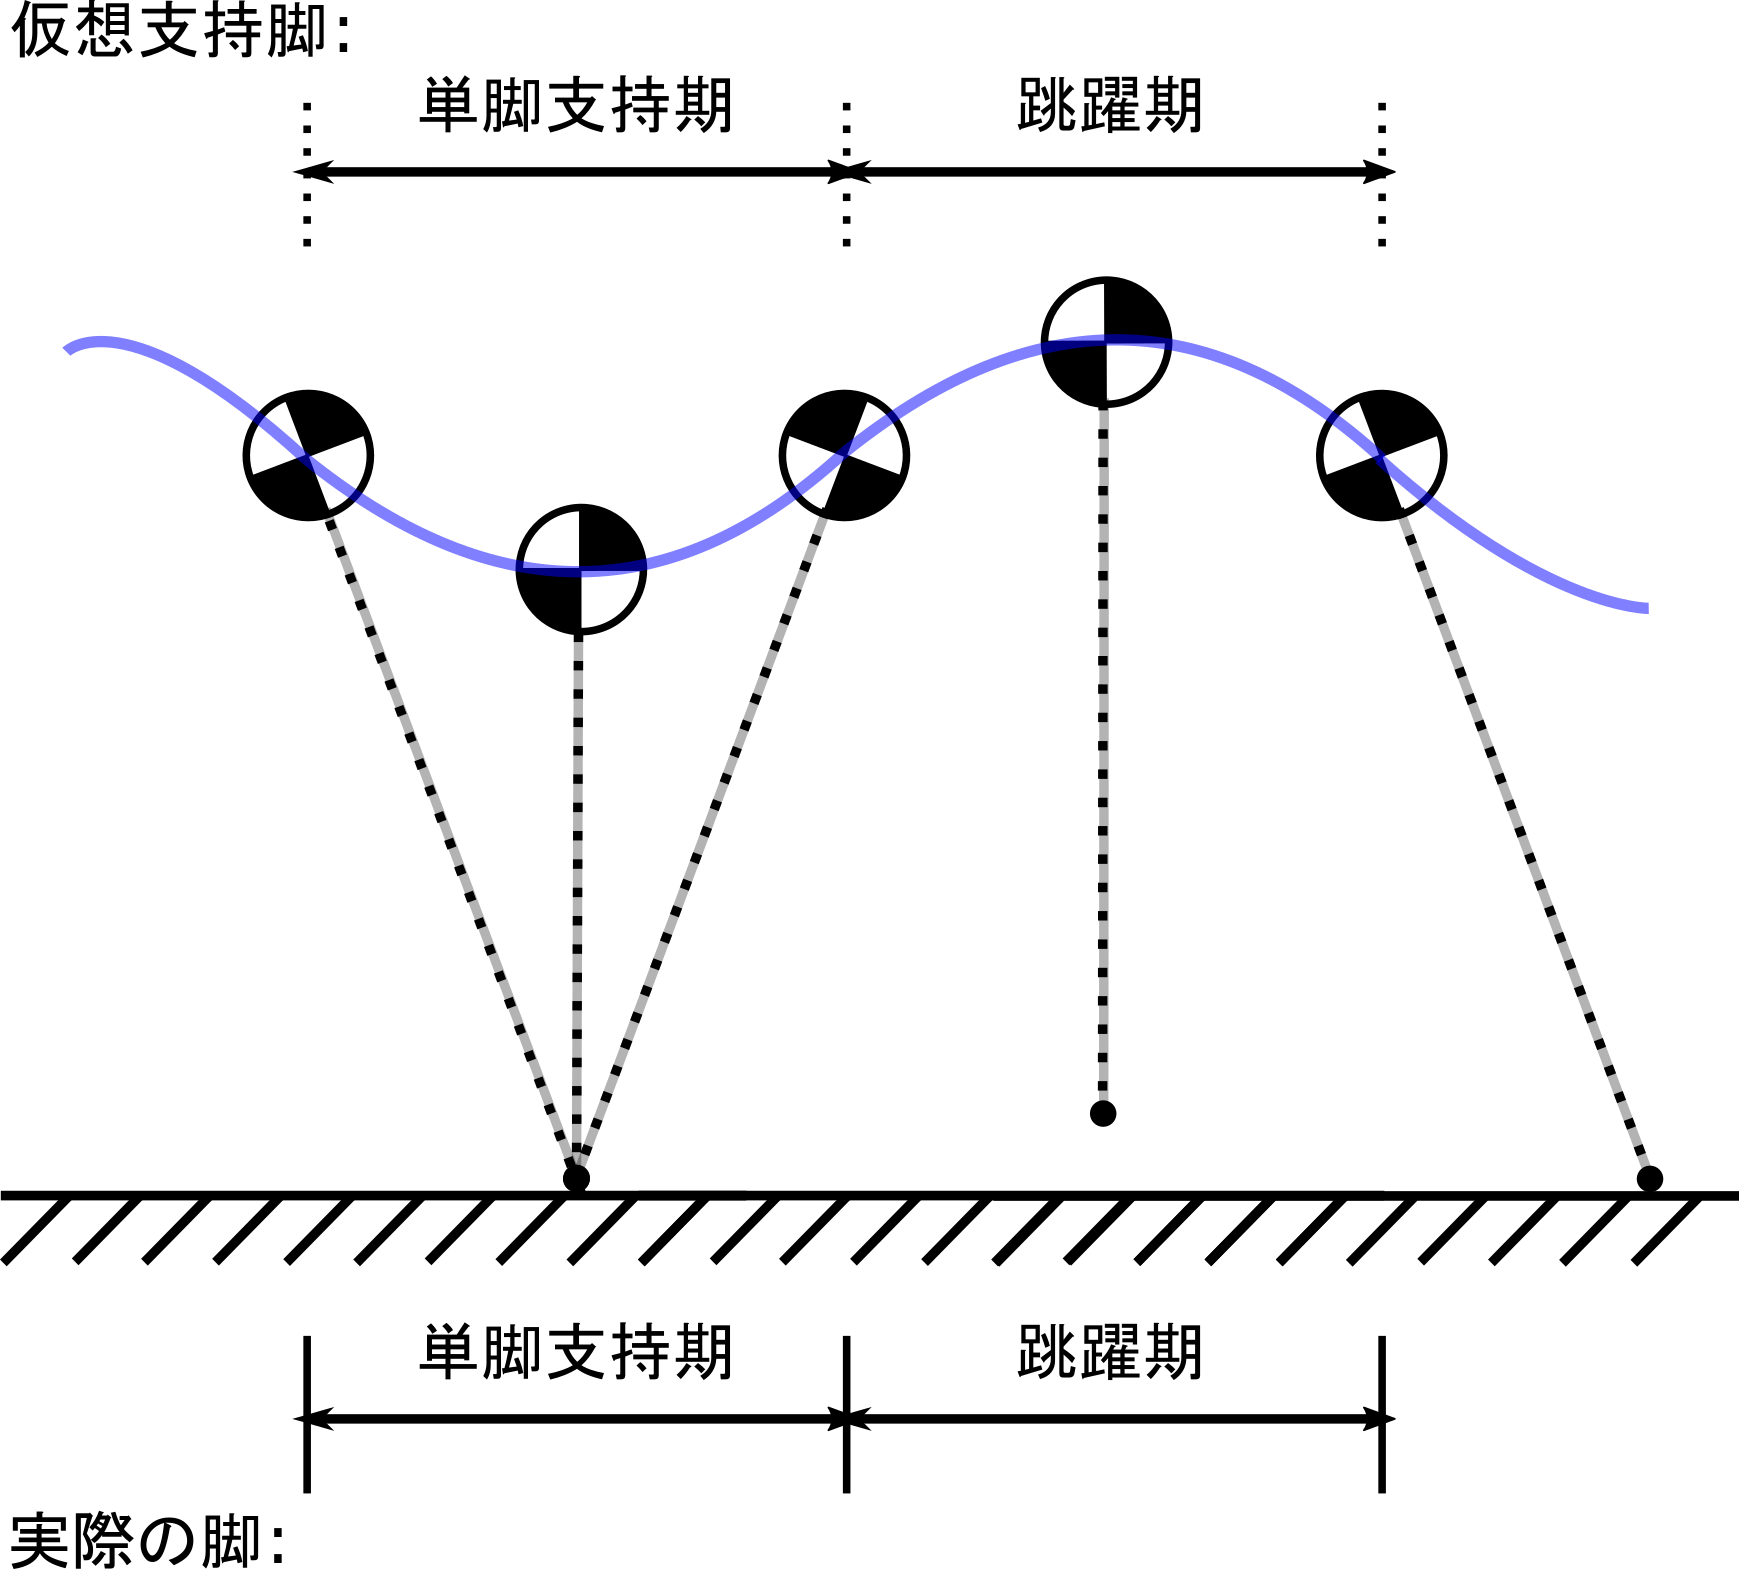
\includegraphics[width = 10.0cm,clip]{./fig/running_with_vsl.png}
 \caption{走行動作に仮想脚を導入した場合.歩行の場合と同様に,青色の曲線は重心軌跡を,黒色の線は脚を,黒色の点線は仮想脚を表している.\label{r_vsl}}
\end{figure}

\begin{figure}[htbp]
 \centering
 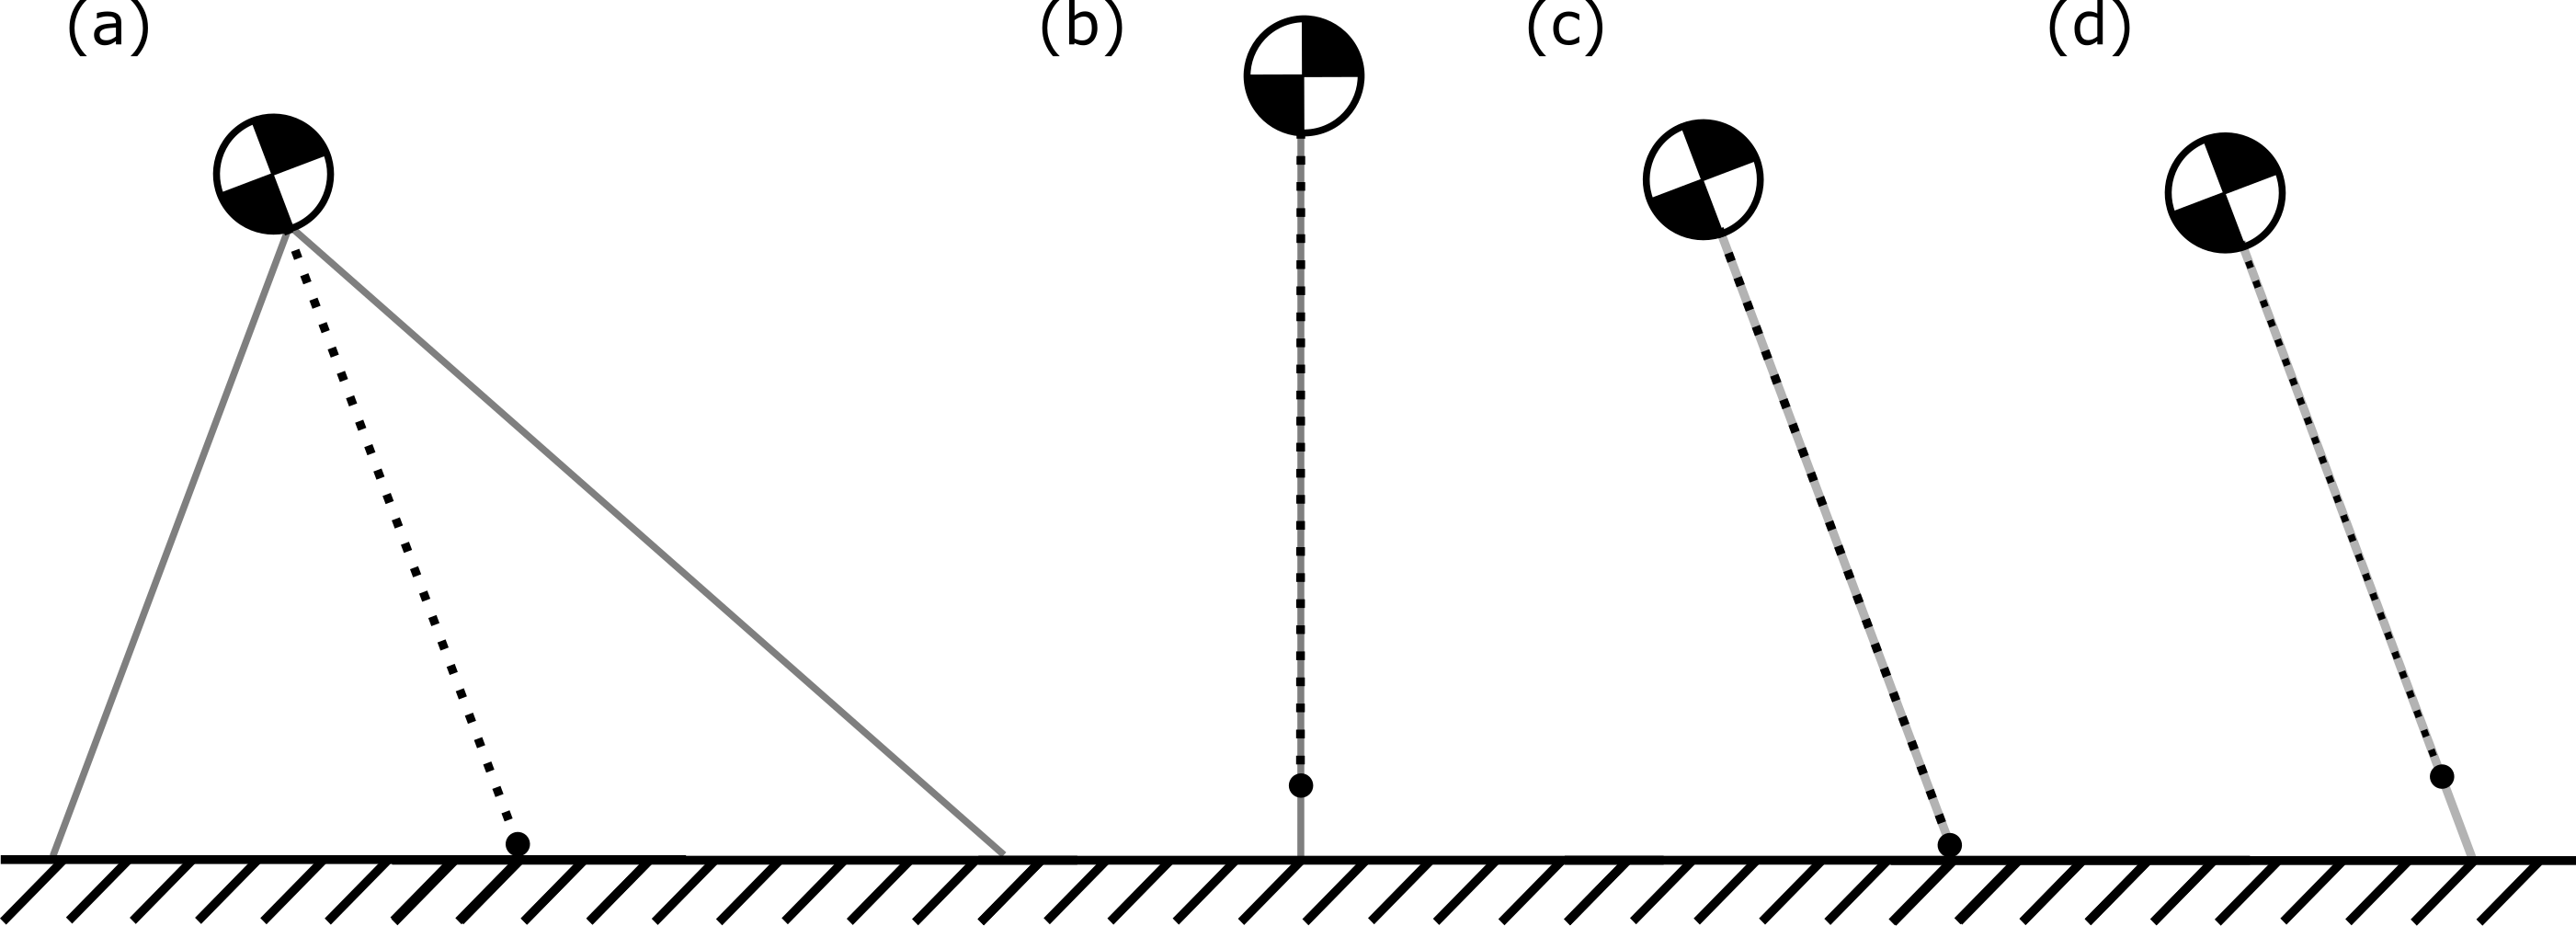
\includegraphics[clip,width=12.0cm]{./fig/vsl_pattern.png}
    \caption{仮想脚と実際の脚がとりうる状態.\label{compare}}
\end{figure}

\begin{table}[htbp]
 \centering
 \begin{tabular}{|l||c|c|c|c|} \hline
     & (a) & (b) & (c) & (d) \\ \hline \hline
    実際の脚 & 両脚支持 & 跳躍 & 単脚支持 & 単脚支持 \\
    仮想脚 & 単脚支持 & 跳躍 & 単脚支持 & 跳躍 \\
 \end{tabular}
\end{table}



\subsection{シミュレーション}

シミュレーションにおける条件として,質量体の質量80[kg],最大時の脚長1.0[m],仮想脚長0.96[m],ばね定数100000[N/m],ダンパ定数1000[Ns/m],目標高さ0.98[m]とし,ばねは脚長が0.97[m]未満のとき作用し,ダンパは現実環境では常に減衰作用が働くことを考慮して,脚長に関わらず作用するようにした.
また,初期条件として,重心位置は水平方向には0[m],鉛直方向には0.2[m]から,水平方向に目標速度を与えた状態で開始する.
この条件で,目標水平速度のみを変化させたときの歩容の変化,重心軌道,水平速度と鉛直速度の推移を観測した.
また,このときの目標水平速度は,0.5m/sから2.0m/sまで,0.5m/sづつ変更することで,モデルの運動の変化を計測した.

以下に,シミュレーションの結果を示す.
Fig.\ref{dx05}とFig.\ref{dx20}はそれぞれ,提案したモデルによる歩行と走行の運動の様子を表している.
また,Fig.\ref{trjdx05}とFig.\ref{trjdx20}はそれぞれ,歩行中,及び走行中の重心軌跡を表している.
横軸,縦軸はそれぞれ水平方向の移動量[m],高さ[m]を表している.

シミュレーションの結果,提案したモデルの目標水平速度を変更するだけで,歩容の遷移が可能であることがわかった.
本実験におけるパラメータでは,目標水平速度1.3[m/s]を境にして,歩行から走行に歩容が変化した.
走行動作においては,いずれの目標水平速度を与えた場合でも,安定な走行状態に収束し,モデルの重心軌道や鉛直方向・水平方向の速度軌跡が一定の波形に収束することがわかった(Fig.\ref{rtrj}).
歩行動作は,走行動作と比較すると,速度軌跡の収束にやや遅れや乱れが見られるものの,走行動作の場合と同様に,重心軌道や速度軌道が一定の波形に収束することができることがわかった(Fig.\ref{wtrj}).




\begin{figure}[htbp]
 \centering
 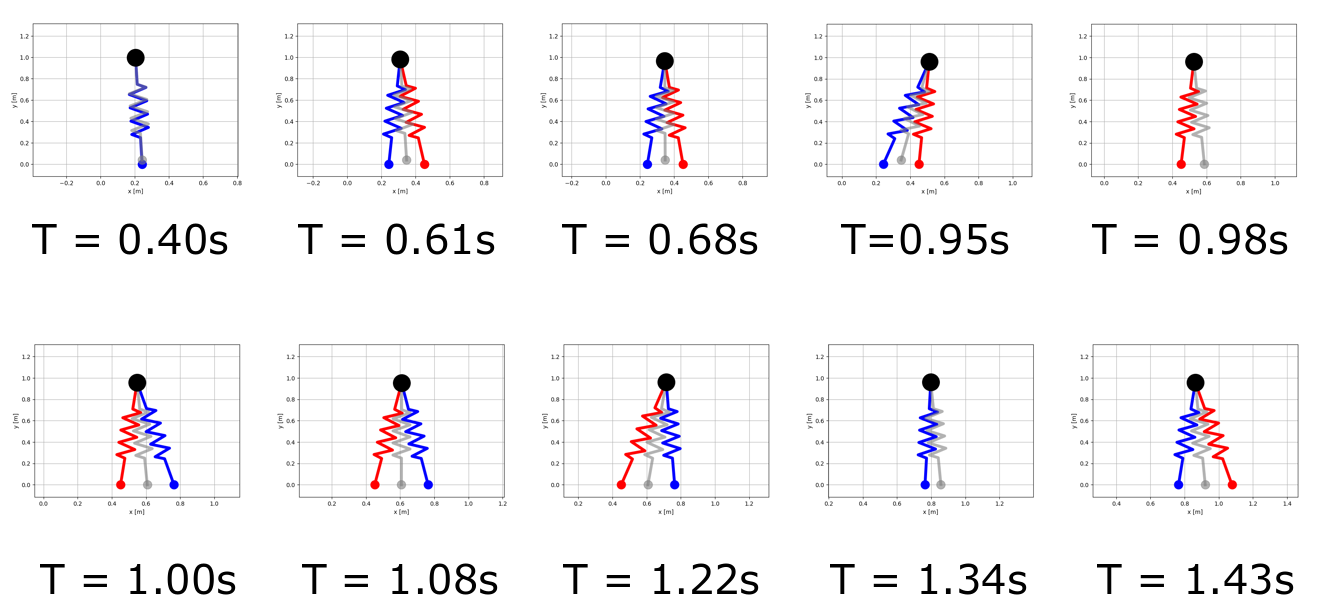
\includegraphics[width = .85\linewidth, clip]{./fig/dx0_5_walking.png}
 \caption{目標水平速度0.5m/sの場合のシミュレーション.\label{dx05}}
\end{figure}
\begin{figure}[htbp]
 \centering
 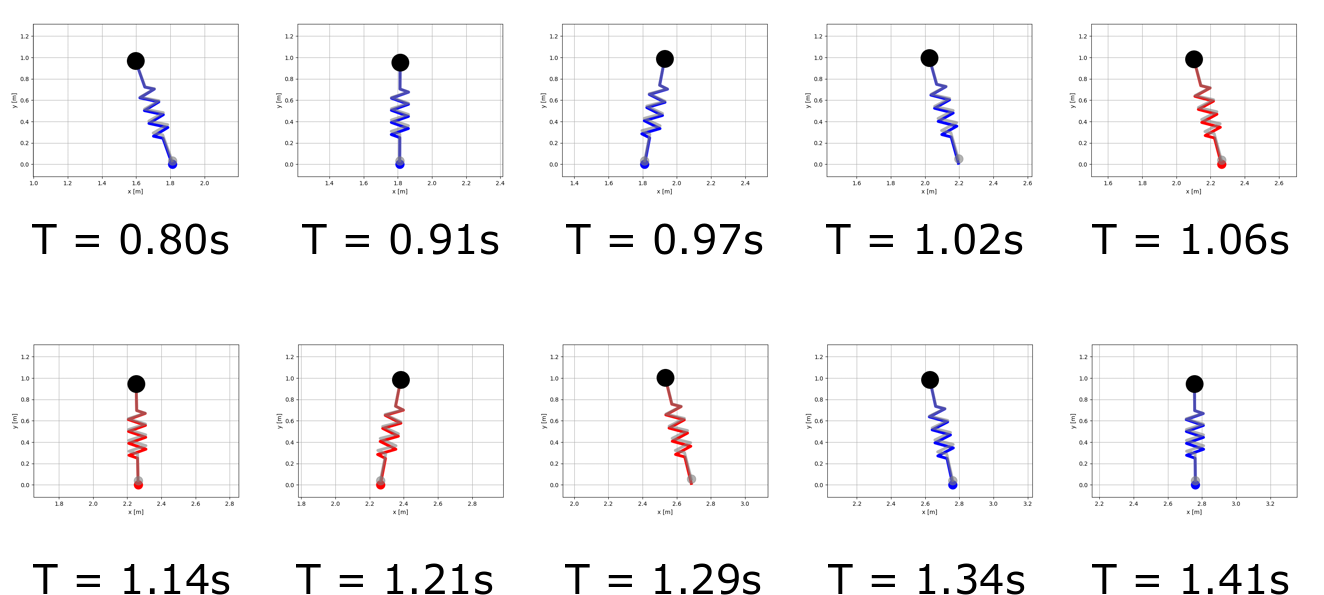
\includegraphics[width = .85\linewidth, clip]{./fig/dx2_0_running.png}
 \caption{目標水平速度2.0m/sの場合のシミュレーション.\label{dx20}}
\end{figure}
\begin{figure}[htbp]
 \begin{minipage}[b]{.5\linewidth}
 \centering
 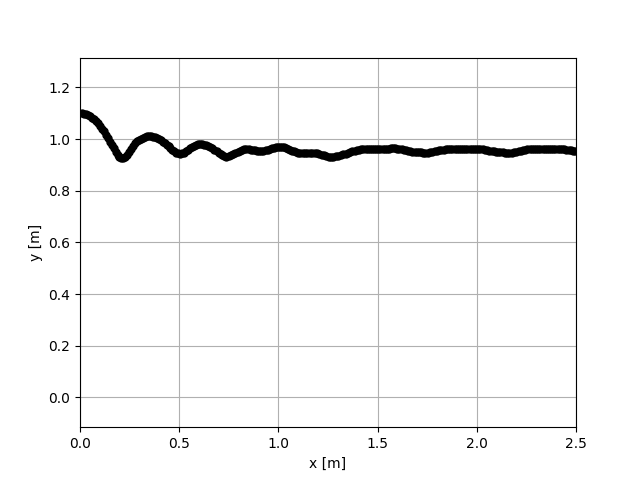
\includegraphics[width = 8cm, clip]{./fig/trj_x2_5_dx1.png}
 \caption{目標水平速度0.5m/s(歩行)の場合の重心軌跡.\label{trjdx05}}
 \end{minipage}
 \begin{minipage}[b]{.5\linewidth}
 \centering
 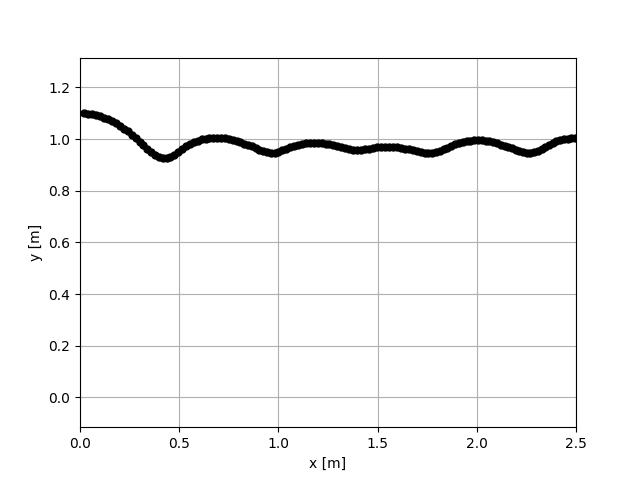
\includegraphics[width = 8cm,clip]{./fig/trj_x2_5_dx2.png}
 \caption{目標水平速度2.0m/s(走行)の場合の重心軌跡.\label{trjdx20}}    \end{minipage}
\caption{歩行と走行における重心軌跡.\label{trj}}
\end{figure}


\begin{figure} % 仮
 \begin{minipage}[b]{.5\linewidth}
  \centering
  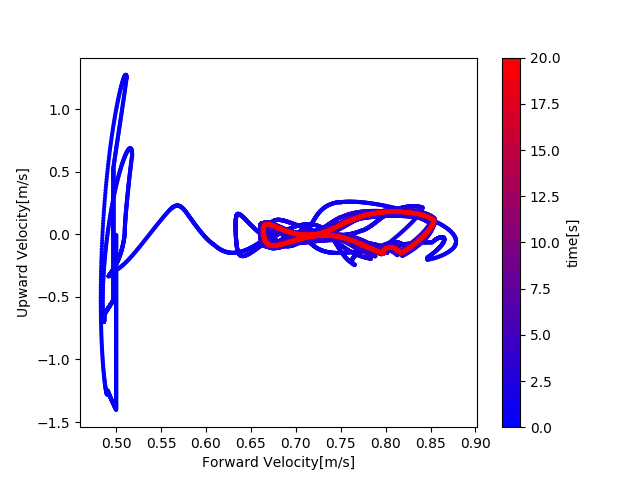
\includegraphics[clip,width = 8cm]{./fig/Velocity_dx0_5walk.png}
  \subcaption{目標水平速度0.5m/sの場合の速度軌跡\label{dxtrj_dx05}.}
 \end{minipage}
 \begin{minipage}[b]{.5\linewidth}
  \centering
  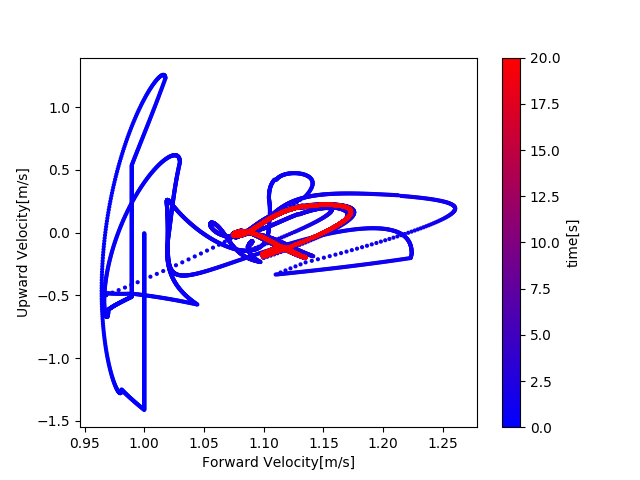
\includegraphics[clip,width = 8cm]{./fig/Velocity_dx1walk.png}
  \subcaption{目標水平速度1.0m/sの場合の速度軌跡\label{dxtrj_dx10}.}
 \end{minipage}
 \caption{歩行時の速度軌跡.\label{wtrj}}
 \begin{minipage}[b]{.5\linewidth}
  \centering
  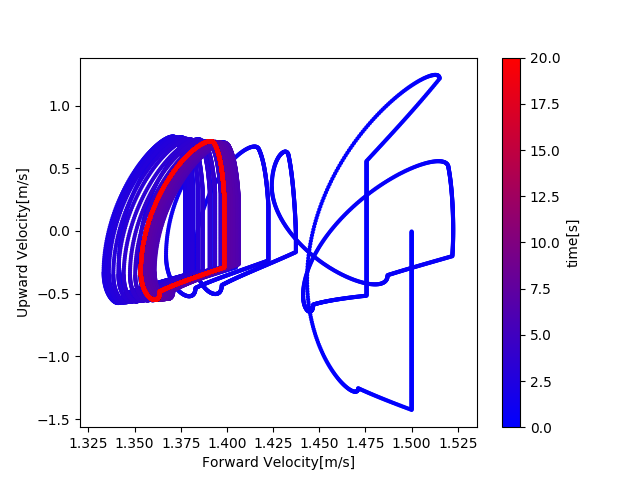
\includegraphics[clip,width = 8cm]{./fig/Velocity_dx1_5run.png}
  \subcaption{目標水平速度1.5m/sの場合の速度軌跡\label{dxtrj_dx15}.}
 \end{minipage}
 \begin{minipage}[b]{.5\linewidth}
  \centering
  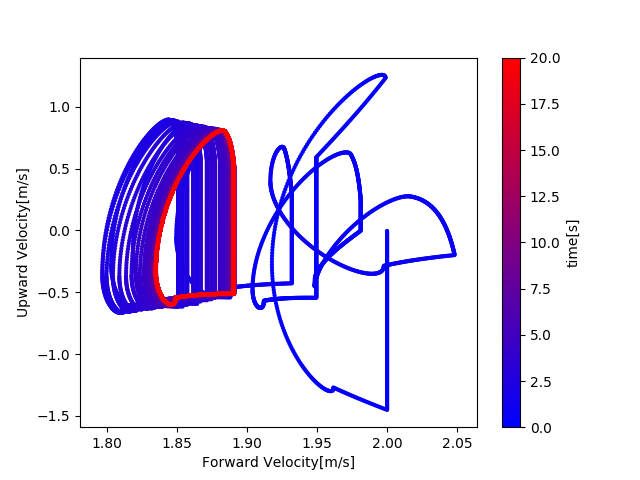
\includegraphics[clip,width = 8cm]{./fig/Velocity_dx2run.png}
  \subcaption{目標水平速度2.0m/sの場合の速度軌跡\label{dxtrj_dx20}.}
 \end{minipage}
 \caption{走行時の速度軌跡.\label{rtrj}}
\end{figure}

\clearpage

\section{2脚ロボット}
本研究で開発した2脚ロボットの外観をFig.\ref{robot_outline}に示す.
ロボットの大きさは,高さ510*幅230*奥行き140[mm],重量2.5[kg]であり,股関節にロールとピッチ方向,膝関節と距腿関節にピッチ方向の自由度をもつ.
股関節の2自由度は,ROBOTIS社製Dynamixel xのサーボモータによって駆動され,膝関節と距腿関節は,マッキベン型空気圧人工筋(以下,空気圧人工筋と呼ぶ)によって駆動される.
また,股関節と膝関節,膝関節と距腿関節の間隔は200[mm]で統一している.
本研究において,使用しているサーボモータは,制御周期20[msec]で角度制御を行っている.
また,空気圧人工筋は,外部のエアコンプレッサによって空気を供給しており,最大で0.6[MPa]給気することが可能である.
空気量を調節する弁にはオンオフ弁を使用し,圧力センサを使用することで圧力制御を行っている.
以下に詳細を述べる.

\begin{figure}[htbp]
\begin{center}
 \includegraphics[clip,width=8.0cm]{}
    \caption{ロボットの外観} % title
    \label{robot_outline}
\end{center}
\end{figure}

\subsection{筋配置}
本研究で使用するロボットには,片脚で4本,合計で8本の空気圧人工筋を使用している.
これらの筋は,ヒトの身体における一関節筋の役割と構造を有している.

\clearpage

\section{実験}
本研究で製作したロボットを用いて,歩行実験を行う.
この実験の目的として,倒立振子モデルの特徴である,

\begin{enumerate}
 \item 支持脚長の変化
 \item 重心軌道
\end{enumerate}

について,歩行中の挙動の解析を目的とする.



\subsection{歩行動作生成}
本研究では,単純な制御によって動くロボットの実現を目的としている.
これを達成するため,ロボットの動作生成手法として,フィードフォワード制御を用いる.
実際には,歩行動作を単純な周期運動であると見なし,あらかじめモータの角度遷移や各筋への給排気パターンを繰り返すという手法を用いる.
ただし,ロボットの初期状態を一定にするため,直立状態を初期状態とし,1歩目のモータおよび空気圧人工筋のパラメータは別の値を用意することとする.

実際に,実験で使用した歩行パラメータパターンをFig.\ref{parameter}に示す.
全ての筋において,給排気の切り替えのタイミングは100msecごとで統一している.
モータの角度は,100msecごとに目標角度値を設定しており,20msecごとに前後の目標角度値の内分点に追従するように動作させている.
また,各筋の給排気パターン及びモータの目標角度値は,実験者が,前述の空気圧人工筋内の圧力値と関節角度の対応を参考に,試行錯誤的に決定したパラメータである.

図の縦の点線は,パラメータの切り替えのタイミングを示しており,1周期を800[msec]に設定した.
横の点線は,1目盛が10[deg]の間隔をとっている.
股関節にあるモータの目標角度について,ピッチ軸は,地面と垂直な状態を0[deg]とし,屈曲を正,伸展を負の角度として設定している.
また,ロール軸も同様に,地面と垂直な状態を0[deg]とし,内転を正,外転を負の角度として設定している.

実際に,Fig.\ref{parameter}の歩行パラメータパターンを用いて,最大4歩の歩行に成功した.
以下に,歩行パラメータの説明を行う.

\begin{description}
\item[支持脚期] \mbox{}
 \begin{enumerate}
  \item 距腿関節と股関節の動作によって,ロボットの重心を大きく前方に倒す.
  \item 重心を前に倒した状態を維持する.
  \item ヒラメ筋を収縮させることで,スムーズな重心移動を実行する.
  \item ヒラメ筋を再び伸長させ,重心移動を慣性によって実行する.
 \end{enumerate}
\item[遊脚期] \mbox{}
 \begin{enumerate}
  \item 距腿関節と股関節の動作によって,ロボットの重心を前方に倒しつつ,次の遊脚を屈曲させる準備をする.
  \item 後ろの支持脚で蹴り出しを行い,そのまま遊脚期に入る.
  \item 遊脚が地面につかないように脚の関節を調節し,脚を前方に大きく振り出す.
  \item 遊脚が支持脚に移行するための準備として,膝関節を伸展状態にさせながら,足部の着く位置を調整する.
 \end{enumerate}
\end{description}
	    
\begin{figure}[htbp]
 \centering
 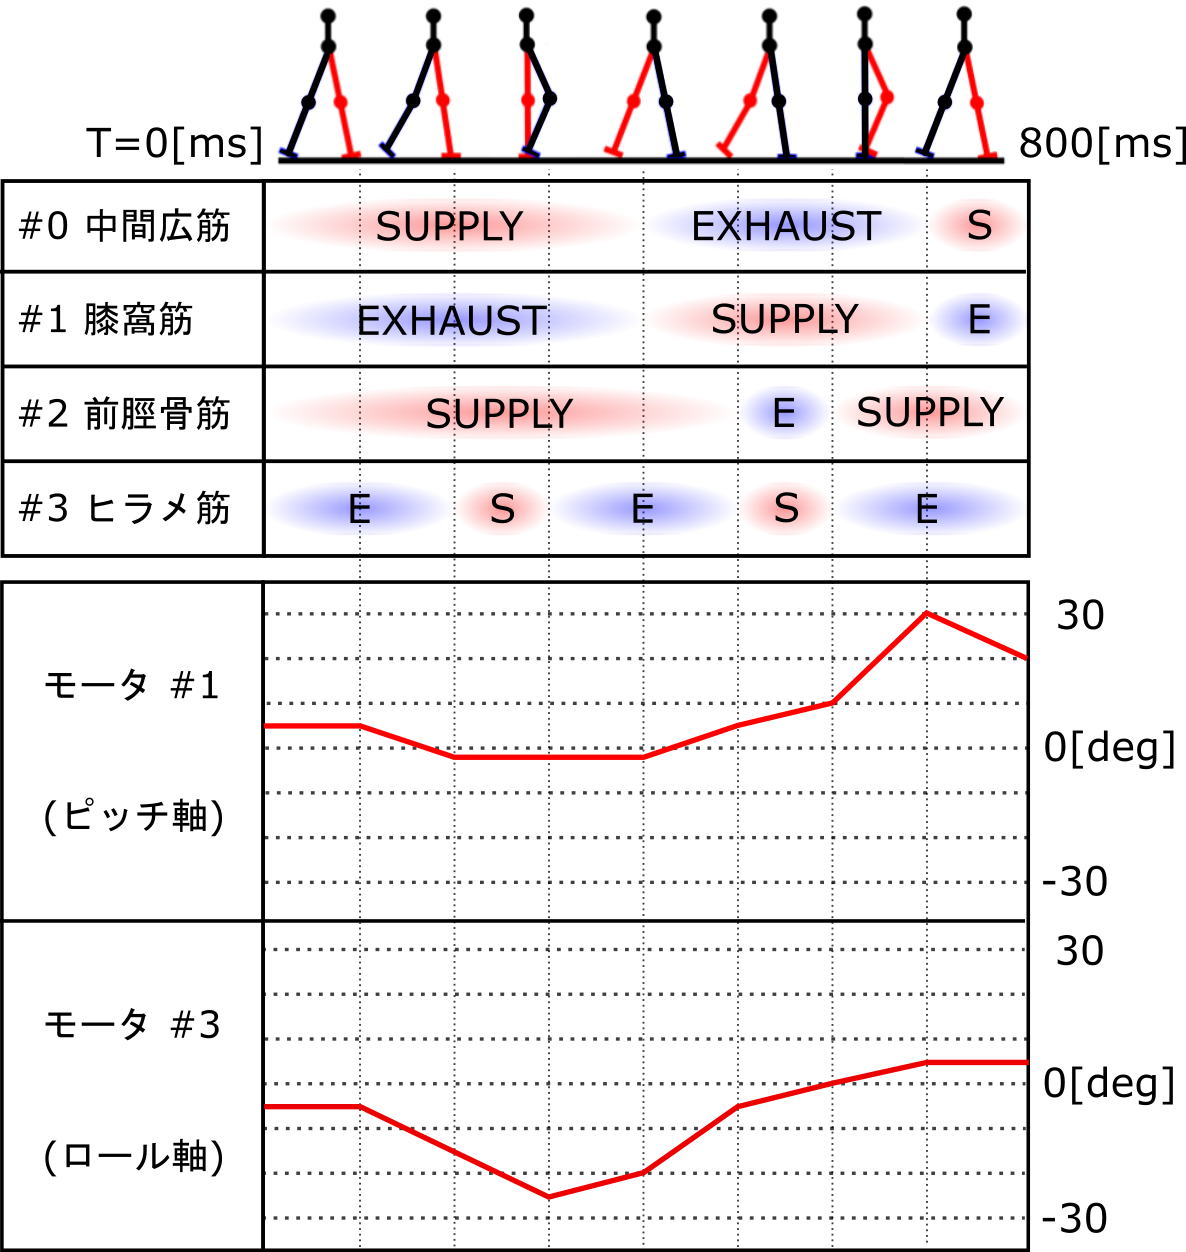
\includegraphics[clip,width=12.0cm]{./fig/parameter_pattern.png}
    \caption{歩行パラメータパターン一覧.図上部の赤く表示された方の脚が,支持脚期から始まる1周期分のパラメータパターンを示している.また,筋のパラメータに書かれているSとEは,それぞれSUPLY,EXHAUSTのことであり,給気と排気を表す.\label{parameter}}
\end{figure}



\subsection{実験環境}
このパラメータを用いて,地面との摩擦を大きくするためにフェルトの布上で歩行実験を行う(Fig.\ref{}).
実験中の試行において,ロボットが最大歩数歩いた実験について,ロボットの関節角度(主に膝関節)の推移と重心移動を計測する.

\subsection{実験結果及び考察}
歩行中のロボットの連続写真をFig.\ref{photoseries}に示す.
本章の始めに述べた,倒立振子モデルがもつ特徴を満たしているかを調べるために,支持脚期における脚の関節角度の推移(Fig.\ref{motioncapture}),及び歩行中の重心位置の推移(Fig.\ref{motioncapture})を,モーションキャプチャを用いて計測した.
また,前者の関節角度の推移については,モーションキャプチャ使用時のマーカ位置によって簡単に確認することができるため,連続写真から分析を行うこととする.

(結果・考察)

\begin{figure}[htbp]
 \centering
 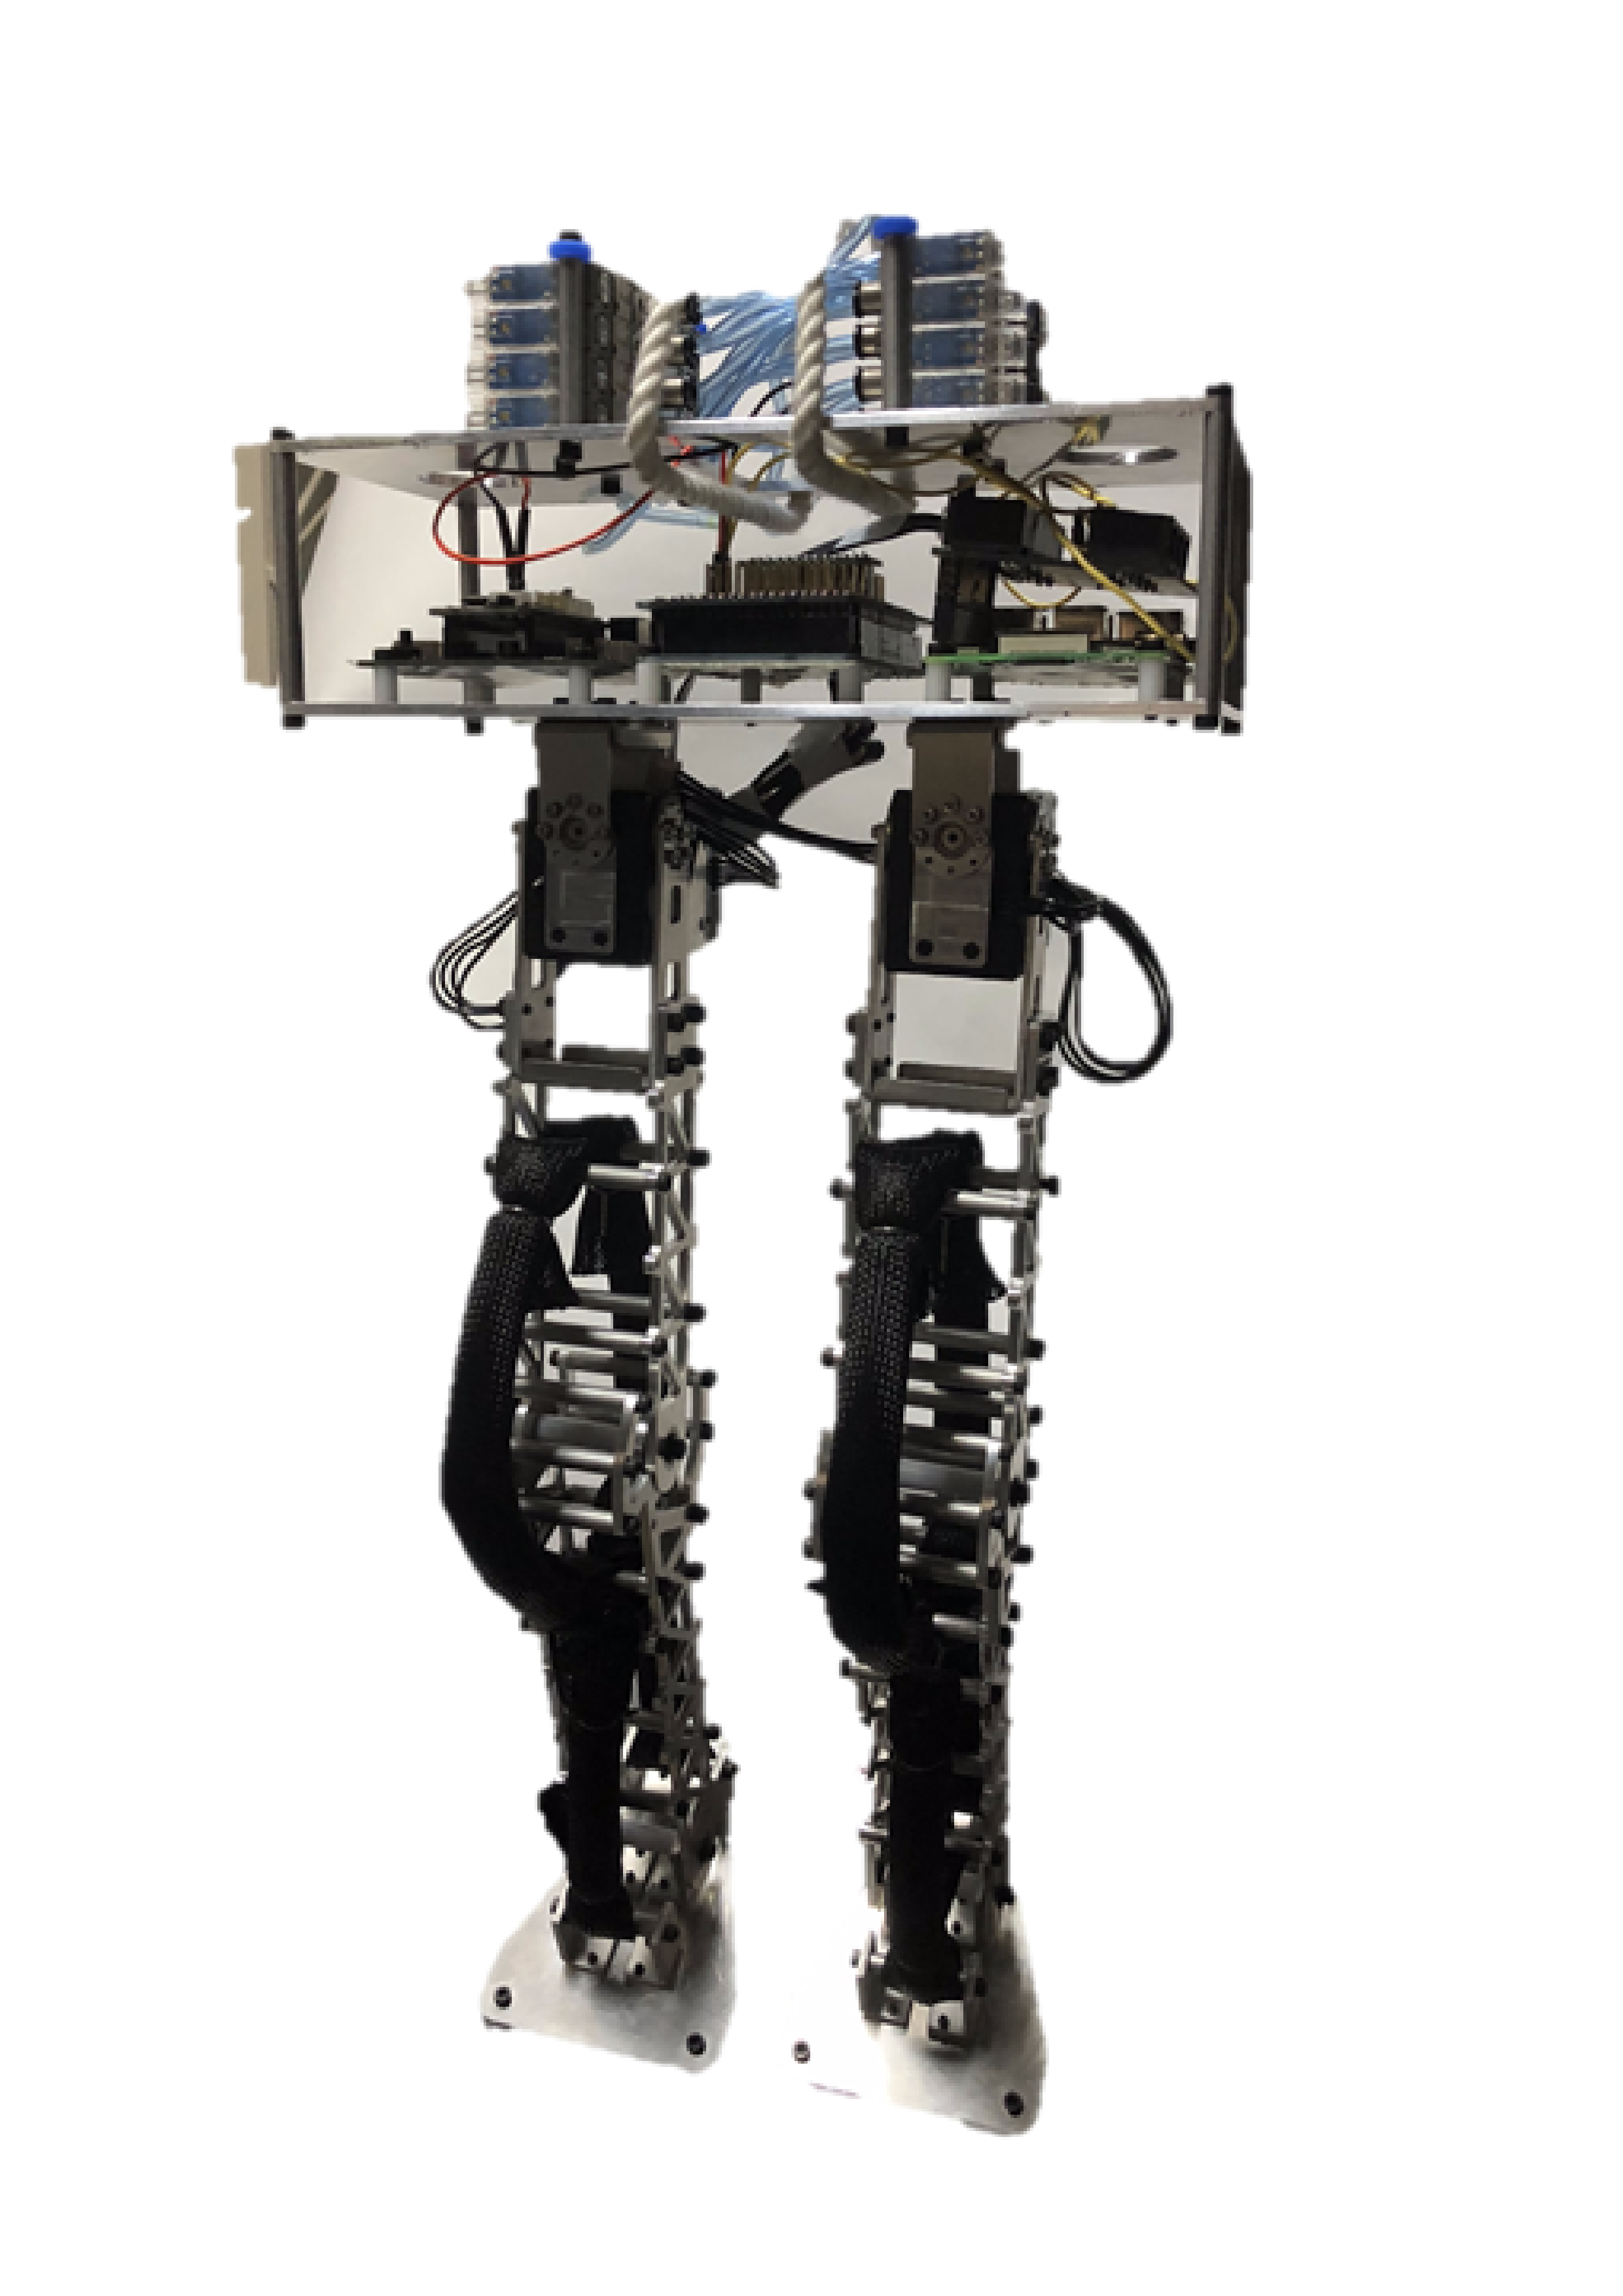
\includegraphics[clip,width=5.0cm]{./fig/robot.png} % 仮
    \caption{歩行中の連続写真.\label{photoseries}}
\end{figure}

\begin{figure}[htbp]
 \centering
 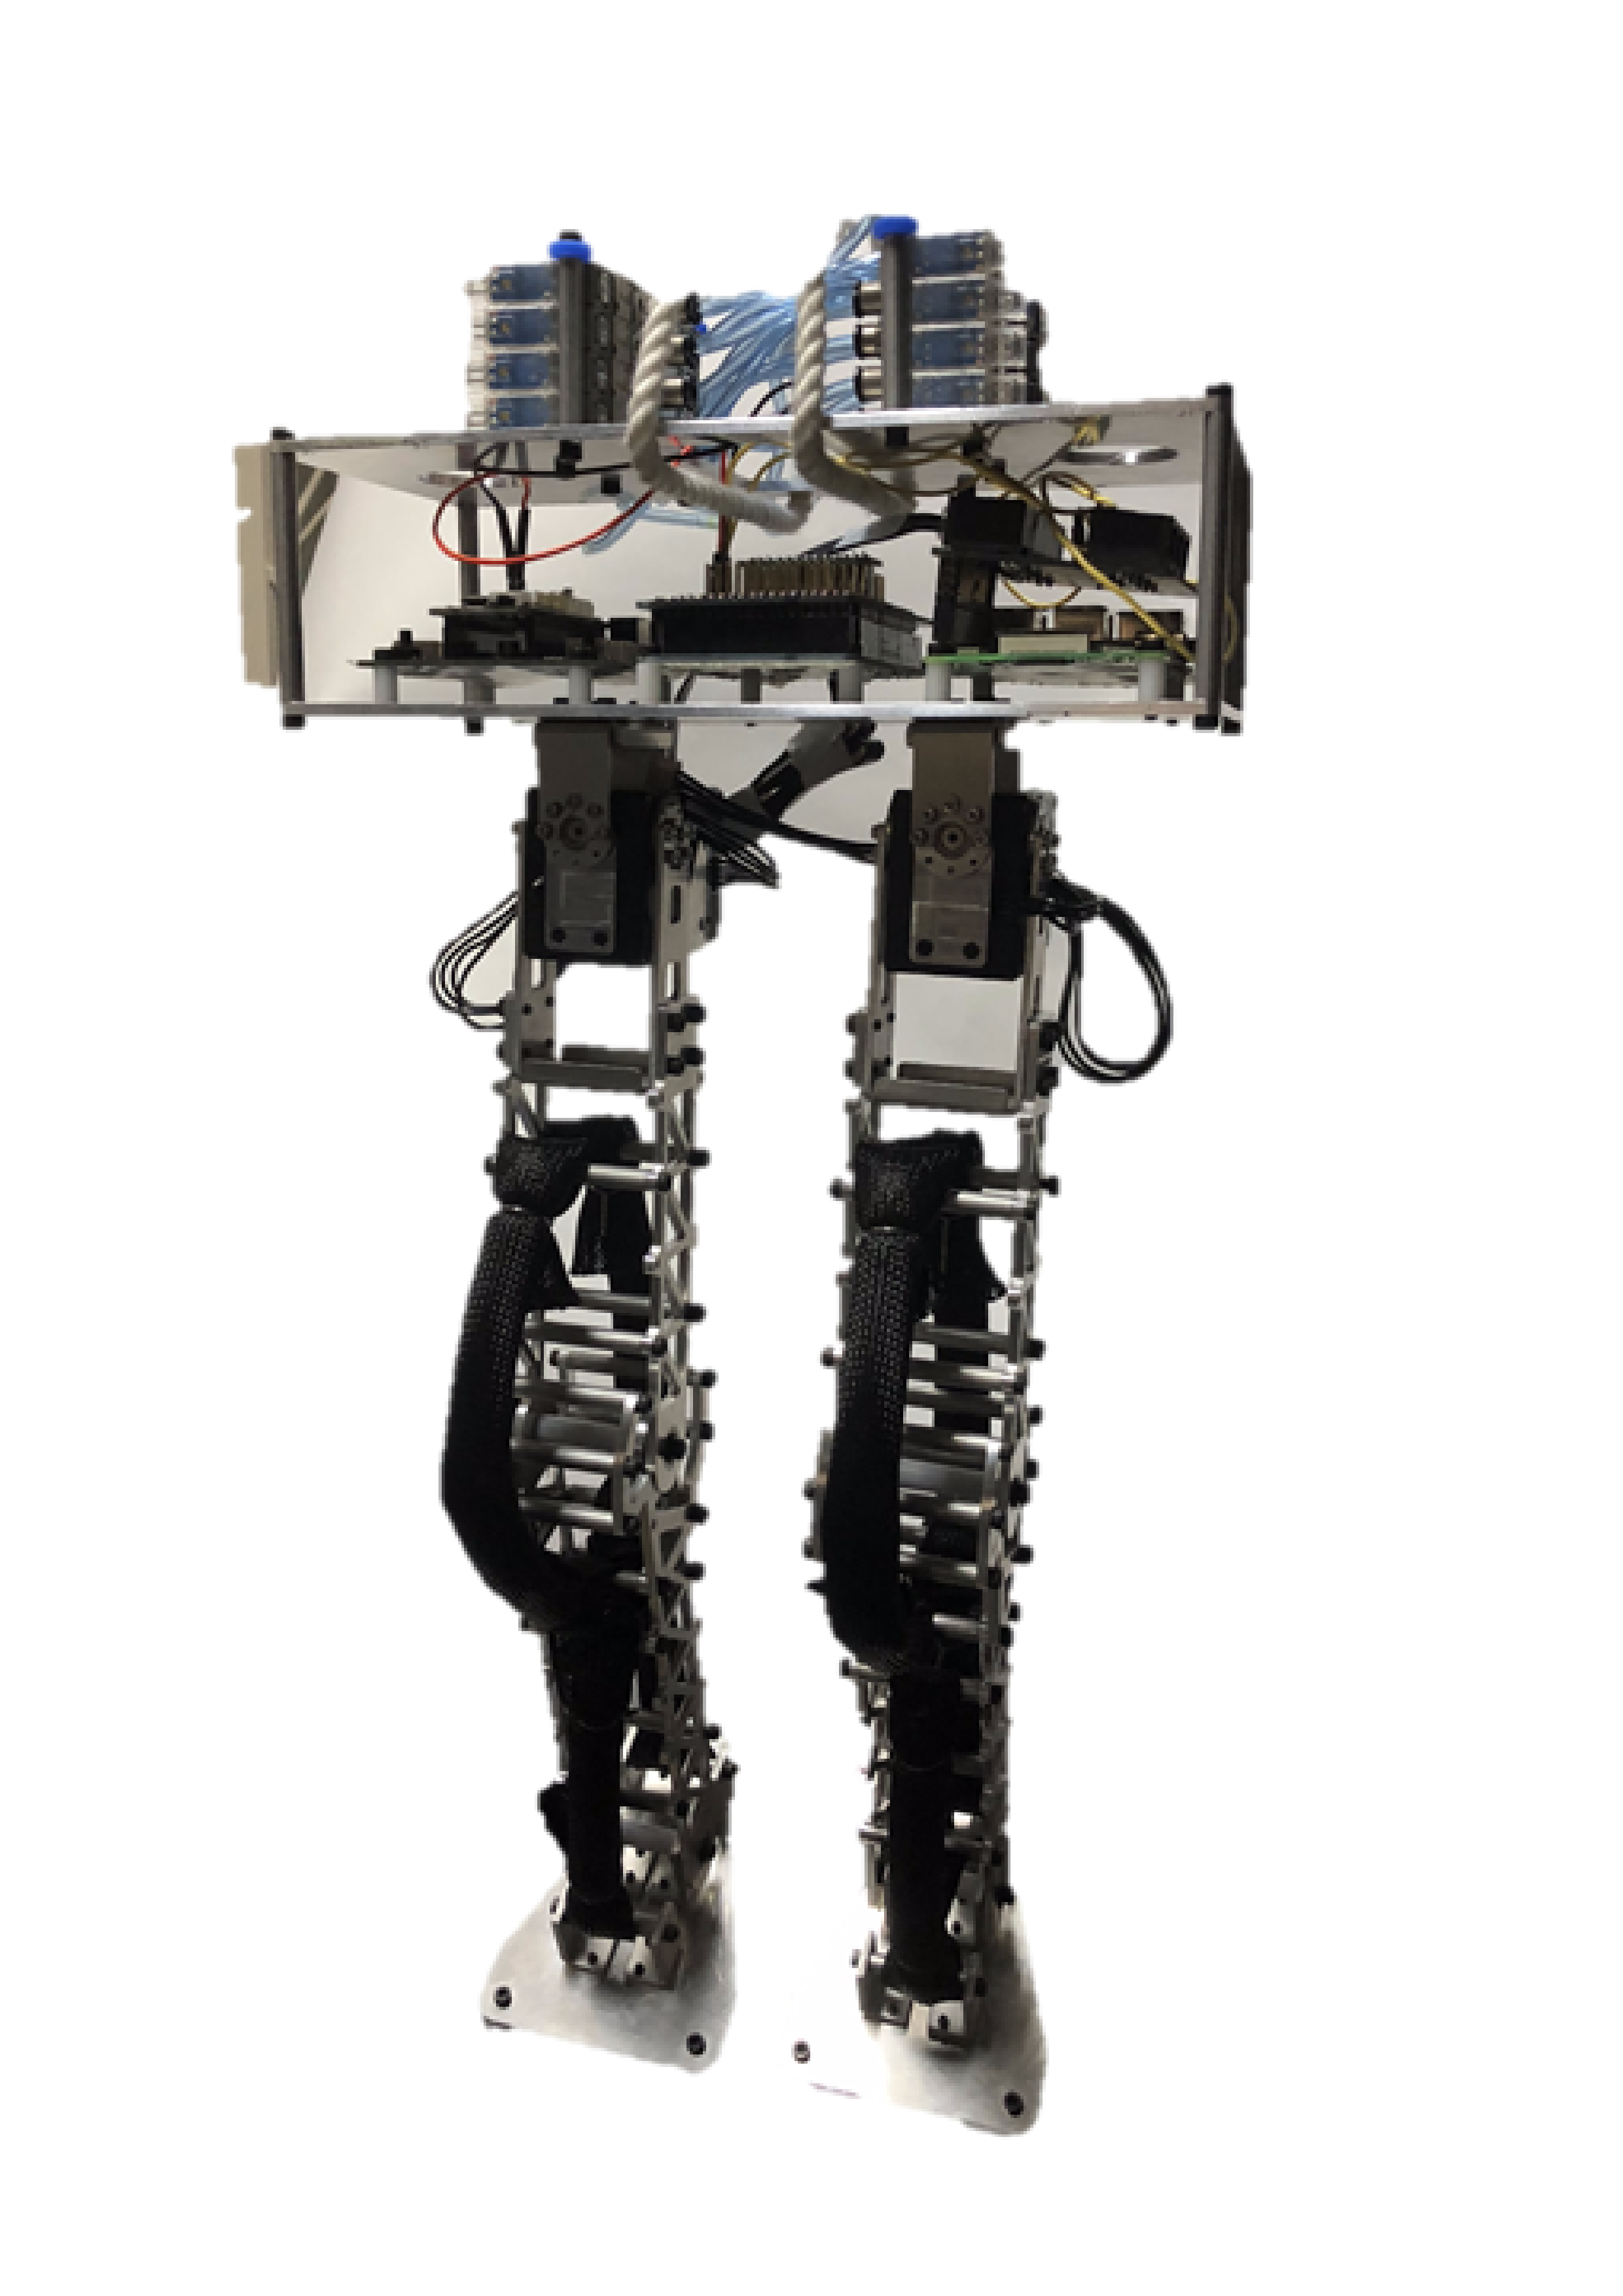
\includegraphics[clip,width=5.0cm]{./fig/robot.png} % 仮
    \caption{モーションキャプチャによる歩行中のロボットのスティック線図.\label{motioncapture}}
\end{figure}

\subsection{走行実験}
本研究では,矢状面方向への速度変化で歩行と走行といった歩容が変化するモデルを提案し,その機構の実装を目標とした.
このため,本ロボットにおいて走行実験も行ったが,走行の一要素である跳躍に必要な力を生み出すことができなかったため,走行を達成することはできなかった.
今回製作したロボットは全長が短く,それに応じて空気圧人工筋の長さも短くする必要があった.
しかし,空気圧人工筋の長さが短いと,収縮長も短くなるため,距腿関節による十分な蹴り出しが行えなかったことが原因であると考えられる.
これを改善するための方法として,距腿関節の底屈に作用する二関節筋である腓腹筋を実装するなどの手法によって,距腿関節の可動域をより大きくすることで改善されるのではないかと考えている.
\clearpage

\section{結論}
本研究では、これまでのモデルでは実現できなかった、歩容の遷移が可能なモデルとその制御則を提案し、それに基づくヒト型二脚ロボットの試作を目的としていた。
われわれはまず、従来の研究で利用されてきた歩行モデルである倒立振子モデルと、走行モデルであるバネマスモデルにおける動作の共通項を調査した。
そこで、剛体脚、ダンパ脚、ばね脚を機構的に切り替えることができるモデルを考案した。
また、脚の自発的動作と受動的動作に着目すると、いずれの歩容においても、重心が描く軌道が一致する点に着目し、仮想支持脚を用いた提案モデルの制御則を使用し、シミュレーションを行った。
さらに、提案したモデルがヒトのような回転軸をもつリンク機構に置き換え、試作したヒト型二脚ロボットによる動作実験を行った。

モデルによるシミュレーションでは、脚モデルの水平方向への目標速度のみを変更可能なパラメータとして、振る舞いの変化を調査した。
実験の結果、目標水平速度を変更するだけで、モデルの歩容を変化させることが可能であることが検証できた。
歩行及び走行中の速度の変化や重心軌道を観察すると、走行時には安定した運動の様子が見られ、歩行時には若干の動作のふらつきが見られたものの、十分な時間が経った場合には、安定して周期的な歩行動作が実現できていることがわかった。

次に、提案した脚モデルをロボットとして実機化するため、2脚ロボットを試作した。
このロボットには、脚構造におけるばね要素とダンパ要素を同時に実現可能な空気圧人工筋を膝関節と距腿関節に使用することで、モデルにおける脚構造の変化や後脚の蹴り出しを実現できるように設計した。
ロボットによる歩行実験を行い、支持脚の状態と重心軌道をモーションキャプチャを用いて調査したところ、モデルのような挙動はあまり実現できていなかった。
また、歩行の実現という点においても、最大3歩までの実現にとどまった。
これらの原因として、ロボットの全長が小さかったために空気圧人工筋の性能を発揮することが難しく、後脚の蹴り出しの力が足りなかったため、ヒトの遊脚の動きを実現できなかった点が挙げられる。
また、走行に関しても同様の理由から、跳躍を行うことができず、動作を実現することが難しかった。
ロボットの筋配置や、今回制御の簡単化の目的から実装しなかった、二関節筋の実装などによって、ロボットの出力不足の問題を緩和できるのではないかと考えている。

本研究におけるモデルの実機化には、改善できる点が多くある。
例えば、試作したロボットでは、モデルにおける重要なパラメータであった水平速度を可視化できるような指標がなかった。
また、ロボットにはほとんどセンサが実装されておらず、外乱や接地などの外部からの信号を検出することはできない。
これらの問題を、ハードウェアやソフトウェアの改善によって解決することで、モデルの動作の再現により近づけることができると考えている。
\clearpage



\Acknowledgment
大阪大学大学院基礎工学研究科システム創成専攻の細田耕教授には,研究方針から論文執筆に至るまで,熱心なご指導,ご鞭撻賜りました.また,すばらしい実験設備を整えていただき,不自由なく研究に励むことができたことに,心より感謝申し上げます.同専攻の清水正宏準教授には,ミーティングなどの場でさまざまなご助言を賜りましたこと,深く感謝いたします.同専攻の池本周平助教には,設計するにあたり並々ならぬ助言,ご指導賜りましたこと,心より感謝申し上げます.先輩方には,研究内容から私生活まで,多くのことについてご助力をいただきました.特に,進さんにはロボットを開発するうえで,ハード面からソフト面にいたるまでご助言ご助力頂きました.心より感謝いたします.研究室の同期生,後輩には,時に考察し合い,時に笑い合い,学んできました.とても有意義な研究生活を送れたこと,深く感謝いたします.特に同じ下肢班の同期生である,梶原くん,藪くんには,頻繁にご助言,ご助力を頂きました.加えて感謝いたします.
\clearpage

\section*{研究業績}
\addcontentsline{toc}{section}{研究業績}
\subsection*{国内会議}
\begin{itemize}
 \item[\labelitemiv] 進寛史,世田竜士,池本周平,細田耕:”股関節と腰関節の連動機能を考慮した2足ロボットの開発”,ロボティクス・メカトロニクス講演会,2017.
\end{itemize}
\bibliographystyle{unsrt}
\bibliography{reference}

\end{document}
